%% This document gives an example on how to use the ntnumasterthesis
%% LaTeX document class.

%% Use short name MACS, MIS, CIMET, MTDMT, MIXD or MIS  
%% Language english or norsk
%% b5paper with oneside or twoside, you can set A4 if you want but you submit in b5

%% If you want print with the heading material on a4 paper you can use this format
%% \documentclass[MACS,english,a4paper,oneside,12pt]{ntnuthesis/ntnuthesis}

%% with the change to using DAIM we have a new option. include DAIM after english below removes the front page material so that you can then submit in the DAIM system. If you are wanting the front material remove DAIM and make sure you fill in the DaimData.tex file.
\documentclass[MACS,english]{ntnuthesis/ntnuthesis}

\usepackage[T1]{fontenc}
\usepackage[utf8]{inputenc}     % For utf8 encoded .tex files allows norwegian characters in the files. This can be dangerous if you change to a differnt editor.
%\usepackage[pdftex]{graphicx, hyperref}   % For cross references in pdf
\usepackage{graphicx}
\usepackage{hyperref}   % For cross references in pdf

\usepackage{svg}  % To use svg images

% For smart references 
%    use \cref{label} and Caption and Number will be added automatically
\usepackage[capitalise,noabbrev]{cleveref} 

\usepackage{color}              % For colouring text 
\hypersetup{colorlinks=true,     
		linkcolor=blue,          % color of internal links (change box color with linkbordercolor)
    citecolor=blue,        % color of links to bibliography
    filecolor=blue,      % color of file links
    urlcolor=blue           % color of external links
		}
\usepackage{csvsimple}  % for simple table reading and display
\usepackage{url}
\usepackage{booktabs}
\usepackage{gnuplottex} %miktex option if using miktex on windows
\usepackage{rotating}


\definecolor{darkgreen}{rgb}{0,0.5,0}
\definecolor{darkred}{rgb}{0.5,0.0,0}

\lstset{        basicstyle=\ttfamily,
                keywordstyle=\color{blue}\ttfamily,
                stringstyle=\color{darkred}\ttfamily,
                commentstyle=\color{darkgreen}\ttfamily,
}

% Include styling for Javascript ES6 and Solidity
% Copyright 2017 Sergei Tikhomirov, MIT License
% https://github.com/s-tikhomirov/solidity-latex-highlighting/

\usepackage{listings, xcolor, color, textcomp}

\definecolor{verylightgray}{rgb}{.97,.97,.97}

\lstdefinelanguage{Solidity}{
	keywords=[1]{anonymous, assembly, assert, balance, break, call, callcode, case, catch, class, constant, continue, constructor, contract, debugger, default, delegatecall, delete, do, else, emit, event, experimental, export, external, false, finally, for, function, gas, if, implements, import, in, indexed, instanceof, interface, internal, is, length, library, log0, log1, log2, log3, log4, memory, modifier, new, payable, pragma, private, protected, public, pure, push, require, return, returns, revert, selfdestruct, send, solidity, storage, struct, suicide, super, switch, then, this, throw, transfer, true, try, typeof, using, value, view, while, with, addmod, ecrecover, keccak256, mulmod, ripemd160, sha256, sha3}, % generic keywords including crypto operations
	keywordstyle=[1]\color{blue}\bfseries,
	keywords=[2]{address, bool, byte, bytes, bytes1, bytes2, bytes3, bytes4, bytes5, bytes6, bytes7, bytes8, bytes9, bytes10, bytes11, bytes12, bytes13, bytes14, bytes15, bytes16, bytes17, bytes18, bytes19, bytes20, bytes21, bytes22, bytes23, bytes24, bytes25, bytes26, bytes27, bytes28, bytes29, bytes30, bytes31, bytes32, enum, int, int8, int16, int24, int32, int40, int48, int56, int64, int72, int80, int88, int96, int104, int112, int120, int128, int136, int144, int152, int160, int168, int176, int184, int192, int200, int208, int216, int224, int232, int240, int248, int256, mapping, string, uint, uint8, uint16, uint24, uint32, uint40, uint48, uint56, uint64, uint72, uint80, uint88, uint96, uint104, uint112, uint120, uint128, uint136, uint144, uint152, uint160, uint168, uint176, uint184, uint192, uint200, uint208, uint216, uint224, uint232, uint240, uint248, uint256, var, void, ether, finney, szabo, wei, days, hours, minutes, seconds, weeks, years},	% types; money and time units
	keywordstyle=[2]\color{teal}\bfseries,
	keywords=[3]{block, blockhash, coinbase, difficulty, gaslimit, number, timestamp, msg, data, gas, sender, sig, value, now, tx, gasprice, origin},	% environment variables
	keywordstyle=[3]\color{violet}\bfseries,
	identifierstyle=\color{black},
	sensitive=false,
	comment=[l]{//},
	morecomment=[s]{/*}{*/},
	commentstyle=\color{gray}\ttfamily,
	stringstyle=\color{red}\ttfamily,
	morestring=[b]',
	morestring=[b]"
}

\lstset{
	language=Solidity,
	backgroundcolor=\color{verylightgray},
	extendedchars=true,
	basicstyle=\footnotesize\ttfamily,
	showstringspaces=false,
	showspaces=false,
	numbers=left,
	numberstyle=\footnotesize,
	numbersep=9pt,
	tabsize=2,
	breaklines=true,
	showtabs=false,
	captionpos=b
}

%
% ECMAScript 2015 (ES6) definition by Gary Hammock
%

\lstdefinelanguage[ECMAScript2015]{JavaScript}[]{JavaScript}{
  morekeywords=[1]{await, async, case, catch, class, const, default, do,
    enum, export, extends, finally, from, implements, import, instanceof,
    let, static, super, switch, throw, try},
  morestring=[b]` % Interpolation strings.
}


%
% JavaScript version 1.1 by Gary Hammock
%
% Reference:
%   B. Eich and C. Rand Mckinney, "JavaScript Language Specification
%     (Preliminary Draft)", JavaScript 1.1.  1996-11-18.  [Online]
%     http://hepunx.rl.ac.uk/~adye/jsspec11/titlepg2.htm
%

\lstdefinelanguage{JavaScript}{
  morekeywords=[1]{break, continue, delete, else, for, function, if, in,
    new, return, this, typeof, var, void, while, with},
  % Literals, primitive types, and reference types.
  morekeywords=[2]{false, null, true, boolean, number, undefined,
    Array, Boolean, Date, Math, Number, String, Object},
  % Built-ins.
  morekeywords=[3]{eval, parseInt, parseFloat, escape, unescape},
  sensitive,
  morecomment=[s]{/*}{*/},
  morecomment=[l]//,
  morecomment=[s]{/**}{*/}, % JavaDoc style comments
  morestring=[b]',
  morestring=[b]"
}[keywords, comments, strings]


\lstalias[]{ES6}[ECMAScript2015]{JavaScript}

% Requires package: color.
\definecolor{mediumgray}{rgb}{0.3, 0.4, 0.4}
\definecolor{mediumblue}{rgb}{0.0, 0.0, 0.8}
\definecolor{forestgreen}{rgb}{0.13, 0.55, 0.13}
\definecolor{darkviolet}{rgb}{0.58, 0.0, 0.83}
\definecolor{royalblue}{rgb}{0.25, 0.41, 0.88}
\definecolor{crimson}{rgb}{0.86, 0.8, 0.24}

\lstdefinestyle{JSES6Base}{
  backgroundcolor=\color{white},
  basicstyle=\ttfamily,
  breakatwhitespace=false,
  breaklines=false,
  captionpos=b,
  columns=fullflexible,
  commentstyle=\color{mediumgray}\upshape,
  emph={},
  emphstyle=\color{crimson},
  extendedchars=true,  % requires inputenc
  fontadjust=true,
  frame=single,
  identifierstyle=\color{black},
  keepspaces=true,
  keywordstyle=\color{mediumblue},
  keywordstyle={[2]\color{darkviolet}},
  keywordstyle={[3]\color{royalblue}},
  numbers=left,
  numbersep=5pt,
  numberstyle=\tiny\color{black},
  rulecolor=\color{black},
  showlines=true,
  showspaces=false,
  showstringspaces=false,
  showtabs=false,
  stringstyle=\color{forestgreen},
  tabsize=2,
  title=\lstname,
  upquote=true  % requires textcomp
}

\lstdefinestyle{JavaScript}{
  language=JavaScript,
  style=JSES6Base
}
\lstdefinestyle{ES6}{
  language=ES6,
  style=JSES6Base
}




%Typesetting of C++ but not always stable in titles etc...
\newcommand{\CPP}[0]{{C\nolinebreak[4]\hspace{-.1em}\raisebox{.1ex}{\small\bf +\hspace{-.1em}+\ }}}

%\usepackage[table]{xcolor}% http://ctan.org/pkg/xcolor
%\usepackage[nomessages]{fp}
%\newlength{\maxbarlen}


\newcommand\databar[3][gray!20]{%
  \FPeval\result{round(#3/#2:4)}%
  \rlap{\textcolor{#1}{\hspace*{\dimexpr-\tabcolsep+.5\arrayrulewidth}%
        \rule[-.05\ht\strutbox]{\result\maxbarlen}{.95\ht\strutbox}}}%
  \makebox[\dimexpr\maxbarlen-2\tabcolsep+\arrayrulewidth][r]{#3}}



\newcommand{\com}[1]{{\color{red}#1}} % supervisor comment
%\renewcommand{\com}[1]{} %remove starting % to remove supervisor comments
% This will appear in text \com{Lecuters comment} and be visible unless you uncomment
% the renewcommand line.

\newcommand{\todo}[1]{{\color{green}#1}} % items to do
%\renewcommand{\todo}[1]{} %remove starting % to remove items to do

\newcommand{\n}[1]{{\color{blue}#1}} % other comment
%\renewcommand{\n}[1]{} %remove starting % to remove notes

\newcommand{\dn}[1]{} % add the d to a note to say that you have finished with it.





% Set to true ONLY if using Harvard citation style
\newboolean{HarvardCitations}
\setboolean{HarvardCitations}{false} % false for computer science, true for interaction design and harvard style


\ifthenelse{\boolean{HarvardCitations}}{%
	\usepackage{natbib} % for Harvard names as citations.
}{%
	\usepackage[numbers]{natbib} % for Vancover numbers in bibliography
}

\newcommand{\q}[1]{\leavevmode\marginpar{\small\em #1}}
\renewcommand{\q}[1]{}


\begin{document}

% for students submitting in the DAIM system this information will not be used.
% their is an option for DAIM submission which removes this information and checks it is B5.
% Removing the DAIM option on the document type will use this material.

\setthesistitle{Implementation of a tournament based distributed lottery on Ethereum}
\setthesisshorttitle{Distributed lottery on Ethereum} % a short version for the page headers if your normal title is too long to fit
\setthesisauthor{Viktor Frede Andersen}
\setthesissupervisor{Letizia Jaccheri}
\setthesissupervisorA{Mariusz Nowostawski}  % if you have a second supervisor add it like this
%\setthesissupervisorB{Prof. Smart Guy}  % if you have a second supervisor add it like this


\nmtkeywords{Thesis, Latex, Template, IMT}
%\nmtdesc{This is the short description of a masters thesis}


\setthesisdate{06-06-2019}
\setthesisyear{2019}



%for CIMET theses you need to see all of these as well

%\setthesiscampus{Gj\o{}vik}
%\setthesisHostInstitution{\NTNU}
%\setthesisHostInstitution{University of Eastern Finland}
%\setthesisHostInstitution{Universit\'e Jean Monnet Saint-Etienne}

%\setthesisjuryA{} %jury names
%\setthesisjuryB{} %jury names
%\setthesisjuryC{} %jury names
%\setthesisjuryD{} %jury names


 % this is the file which contains all the details about your thesis
\makefrontpages % make the frontpages
%this is the intro to the thesis
%\thesistitlepage % make the ordinary titlepage
\hypersetup{pageanchor=false}
%\include{summary}

\chapter*{Preface}
%Here, you give a brief introduction to your work. What it is (e.g., a Master's thesis in AIMT at NTNU, when it was carried out (e.g., during the autumn semester of 2021). If the project has been carried out with a company, you should mention this and also describe the cooperation with the company. You may also describe how the idea to the project was brought up.

%You should also specify the assumed background of the readers of this report (who are you writing for).\\[2cm]

This is a Master's thesis carried out during the spring semester of 2019 for the completion of the 5-year computer science program at \NTNU, Trondheim.
The idea for a tournament based lottery on Ethereum was inspired by the works of Miller and Bentov and Bartoletti and Zunino. The search for a thesis went over a long time during which I studied blockchain applications and learned about the blockchain space.

The readers of this report are assumed to have a background in computer science with some knowledge of distributed systems and blockchains.

\begin{center}
%\thesiscampus, 
\thesisdate \\[1pc]
%\\[1pc]
\thesisauthor
\end{center}
\chapter*{Acknowledgment}

I would like to thank the following persons for their great help during the thesis work:

\noindent
Mariusz Nowostawski for being an excellent supervisor and mentor with patience and understanding.

\noindent
My mom Liv Unni Andersen and dad Jan Kjetil Andersen for mental support, guidance, and for pushing me when progress was slow.

\noindent
All contributors to the academic work which I built this thesis on, including open source contributors and advocates of Bitcoin, Ethereum, and associated software projects.


%I would like to thank the following persons for their great help during \ldots

%If the project has been carried out in cooperation with an external partner (e.g., a company), you should acknowledge the %contribution and give thanks to the involved persons.

%You should also acknowledge the contributions made by your supervisor(s).

\begin{flushright}
V.F.A.\\[1pc]
\end{flushright}
\chapter*{Abstract}

%This is a summary of the thesis including the conclusion of what was discovered.
Distributed lotteries on the internet is an interesting application with uses in gambling and other areas. Blockchains that function as smart contract platforms can be used to both transfer value and enforce protocols for multiparty computing without relying on a trusted intermediary. This has made it possible to design lotteries with verifiable randomness and with a guarantee of successful completion. 

One promising design of a distributed lottery on a blockchain is based on a tournament of digital coin tosses. This thesis explores the feasibility of such a lottery through making an implementation and doing measurements. The implementation is made for the Ethereum blockchain, which is currently the leading platform for applications using smart contracts. The lottery is assessed by measuring transaction costs and transaction demand, as well as by discussing the security of the lottery in the context of known security issues for blockchain applications and web applications.

We successfully implement a lottery prototype which is likely to work for up to about 100000 participants. Several directions of further research to improve the scalability are identified and discussed. We find that the most concerning security issue is transaction censorship by a powerful collusion of opportunistic miners, which might be an issue for lotteries with a very large prize.

\hypersetup{pageanchor=false}
\chapter*{Abbreviations}

P2P = Peer-to-Peer \newline % 1
PoW = Proof-of-Work \newline % 2
VRF = Verifiable Random Function \newline % 3
PRNG = Pseudo-Random Number Generator \newline % 4
API = Application Programming Interface \newline % 5
MPC = MultiParty Computation \newline % 6
BVM = Bitcoin Virtual Machine \newline % 7
EVM = Ethereum Virtual Machine \newline % 8
CA = Contract Account \newline % 9
EOA = Externally Owned Account \newline % 10
dApp = Decentralized Application \newline % 11
RPC = Remote Procedure Call \newline % 12
DoS = Denial-of-Service \newline % 13
PoS = Proof-of-Stake \newline
HDS = Hierarchical Deterministic Secrets \newline


\tableofcontents

\hypersetup{pageanchor=true}

% Comment with a percent to remove figures or tables:
\listoffigures
\listoftables
\lstlistoflistings


\chapter{Introduction}
\label{chap:introduction}

A lottery can be defined as a random distribution of a prize fund to a set of participants, or random selection of a subset of winners from a larger set of participants to receive some privilege. A lottery is often associated with its use is gambling where one becomes a participant by contributing to a prize fund by buying a ticket, whereupon a set of winning tickets is randomly drawn and a part of the fund is redeemable by owning a winning ticket. Lotteries have also been used in important societal functions such as leader election in democratic governance \cite{sintomer_random_2010} or proof-of-stake systems, drafting of soldiers to war \cite{nixon_executive_1969}, randomized audit controls [Taiwan Uniform Invoice Lottery], and distribution of scarce goods [Shanghai license plates], or as a game used in conjunction with fundraising to a charitable cause. 

Since the stakes in a lottery can be quite high, as with large cash prizes or being drafted to a war, it is important that the result is unpredictable and unbiased. For the lottery achieve its purpose of ultimately distributing the prize, it is important that there is consensus of the result, and that the rules are enforced. Achieving unbiased randomness and consensus is typically done in one of two ways: 1) auditing and public verification of every step of the protocol, i.e. paper tickets being sold and blindly drawn from a basket, as is common for small-scale charity lotteries, and 2) trust in a central authority to conduct the lottery fairly and according to the rules, which is typical for national lottos and government-initiated lotteries. Due to scalability issues, auditing and verification of the second type are often done by a third party such as government or industry inspectors.

With the advent of the internet and peer-to-peer (P2P) online communications, it is natural to explore the possibility of porting lotteries to this domain. While lotteries that use trusted parties and/or centralized authorities can be ported to an internet setting, the subject of this review is internet based lotteries that minimize trust and centralization, which we call \emph{P2P lotteries}. Research has been done on lotteries and coin tosses in a distributed setting in relations to the problem of byzantine consensus \cite{broder_provably_1985}, and various lottery protocols make trade-offs in communication overhead, security models, speed, fault-tolerance, etc. Various breakthroughs in cryptography and distributed computing have been applied to lotteries such as delay functions \cite{goldschlag_publicly_1998}, weakly encrypted secrets \cite{syverson_weakly_1998}, shared decryption keys \cite{fouque_sharing_2001}, distributed hash tables \cite{grumbach_distributed_2017}, and symmetric bivariate polynomials \cite{xia_information_2019}. Of particular interest are P2P lotteries implemented on blockchain platforms such as Bitcoin and Ethereum, as they provide a platform for secure multiparty computing \cite{andrychowicz_secure_2014} and value transfer in a trustless manner not seen with different consensus mechanisms [Bitcoin backbone paper??]. Several designs of blockchain based lotteries have been proposed in peer-reviewed articles \cite{bartoletti_constant-deposit_2017} \cite{miller_zero-collateral_2017} \cite{andrychowicz_secure_2014} \cite{liao_design_2017} \cite{back_note_2014}, and others have been implemented as smart contracts \cite{ago_fairlotto_2018} \cite{noauthor_smartbillions_nodate} \cite{noauthor_satoshi_nodate}.

Blockchain platforms with cryptocurrencies mark an important shift in p2p computing, as they make it possible to transfer value and arrive at global consensus without a trusted intermediary. Due to scripting capabilities of several blockchain platforms, it is also possible to implement a number of financial instruments and games involving money. There have been gambling and lottery applications on Bitcoin and Ethereum for some time, and the topic of lotteries has been discussed in the academic literature. One class of lotteries uses digital coin tosses organized in a tournament to fairly select a winner. This scheme can in theory support a large amount of participants while also maintaining a high degree of resistance from collusion and verifiability of the entire lottery process.

A lottery of this sort has as far as we know been implemented as a proof-of-concept, but not been analyzed and discussed in detail. Applications of smart contracts have to cross a gap from theoretical soundness to practical feasibility. By analyzing an implementation in detail, measure its cost to deploy, and discuss its security and other issues, we hope to get a better understanding of lotteries on a blockchain.

\section{Thesis statement}
\label{sec:statement}

Miller and Bentoc in \cite{miller_zero-collateral_2017} outline a fair lottery that can be implemented both on the Bitcoin platform and on other blockchains with a more expressive scripting language such as Ethereum. The authors note that an implementation of their lottery on Ethereum is significantly less complex and more scalable than the same scheme on Bitcoin. For this reason, as well as the fact that Ethereum has a rich ecosystem of developer tools and user interfaces that make smart contract applications accessible, we decided to implement a full version of the lottery on Ethereum. 

Although there exist several lotteries on Ethereum already, to our knowledge none fulfill the security requirements of Miller and Bentov's lottery. The purpose of creating an implementation is to get some insight into the viability of the lottery in a practical sense. While we will discuss theoretical considerations for the lottery, we expect to discover new considerations related to security, usability, and performance with a working implementation. 

What can we learn from implementing a lottery on Ethereum? What can we say about the security of such a lottery if implemented on a blockchain?

\section{Methodology}
\label{sec:methodology}

\subsection{Literature review}

A systematic literature review on p2p lotteries was conducted prior to writing this thesis in order to place the work in the context of published literature. Sources were collected by conducting a keyword search in online databases for published academic papers. The results from the search were restricted to the fields of computer and information science, as there were many irrelevant hits from different fields. All papers that included a design of a distributed lottery were included in the review. Further relevant works were found in the reference list of papers found through the keyword search. 

\begin{table}[h]
\centering
\caption{Keyword search on Scopus}
\begin{tabular}{|l|l|l|l|}
\hline

term & hits & filtered hits & lottery designs \\ \hline
Term 1 & 13 & 12 & 7 \\ \hline
Term 2 & 44 & 20 & 14 \\ \hline

\end{tabular}
\end{table}
\emph{Table of results from literature search. See terms below.}

\begin{itemize}
    \item Term 1: (bitcoin OR blockchain) AND (lottery OR lotteries) 
    \item Term 2: (verifiable OR verifiability OR p2p OR "peer-to-peer" OR distributed) AND (lottery or lotteries)
\end{itemize}

\begin{table}[h]
\centering
\caption{Designs of lottery schemes}
\begin{tabular}{|l|l|l|l|}
\hline

from keyword search & from references & total \\ \hline
19 & 6 & 25 \\ \hline

\end{tabular}
\end{table}

\subsection{Data collection}

A working implementation of a distributed lottery was implemented on a local version of the Ethereum blockchain. This is a proof-of-concept application that can be simulated and interacted with in order to collect data and get a sense of what a live implementation would look like. 
We collected data of transaction costs necessary to set up a lottery of various sizes by measuring the gas usage of simulations. 
We found the number of interactions a participant in the lottery is needed to have with the blockchain in order to complete the process successfully. By combining this with common threat models and security assumptions about blockchains, we conducted a detailed discussion on the viability of a large lottery on a blockchain.

\subsection{Data analysis}


\chapter{Background}
\label{chap:background}

\section{Cryptography}
\label{sec:cryptography}

\subsection{Hashing}

All applications of hash functions in this work will use secure hash functions as defined in \cite[p.~153-156]{lindell2014introduction}. For clarification, we will use the term \emph{message} for the input to a hash function and \emph{hash} as the output. In addition to fixed-length and deterministic outputs, the key property of secure hash algorithms is \textbf{collision resistance}. Collision resistance means that it is infeasible for any probabilistic polynomial-time algorithm to find two a message $m' \neq m$, so that $Hash(m') = Hash(m)$. An informal definition of a one-way, or preimage resistant, hash function is that if given a hash h, it is infeasible for a probabilistic polynomial time adversary to find a message m so that $Hash(m) = h$. It is implicit that collision resistant hash functions are also preimage resistant, as finding a collision given a hash is the same as finding the preimage of the hash. \cite[p.~156]{lindell2014introduction}

Hash functions have many uses in various fields, but this paper will focus on the uses in content addressing and cryptography. Content addressing is used in distributed hash tables which is essential to many decentralized file sharing networks, including IPFS and Bittorrent. Cryptographic uses of hash functions in this paper will be about verifying message integrity, preserving immutability, and digital signatures. Hash functions are also essential to proof-of-work, as a hash with certain properties can be provably difficult to find. \cite{dwork1992pricing}

\subsubsection{Verify message integrity with hashing}

An example from file sharing will be used to demonstrate how to verify a message with hash functions. Bob wants file m, and Bob knows $h = hash(m)$. Alice sends Bob a message $m'$ she claims to be $m$, but Bob does not trust Alice. In order to verify that $m' = m$, Bob can calculate $h' = hash(m')$, and compare it to $h$. If $h = h'$ Bob can be certain that $m = m'$ without needing to trust Alice. 

\subsubsection{Message authentication with hashing (HMAC)}

Parties communicating over an insecure channel with a shared secret can use Message Authentication Codes (MAC) to prove integrity and authenticity of a message. \cite[p.~158--164]{lindell2014introduction}


\subsubsection{Preserving immutability with hash functions}

Hashes can be used to verify messages of arbitrary size when the verifier is able to compute the hash of the message. Data structures such as Merkle trees and blockchains use hashes to link separate pieces of information together, so that a verifier is able to verify the integrity of a message without calculating its hash all at once. 

Let's use an example from blockchains to demonstrate this. A block of height h contains the hash of its parent, the block of height h-1. This makes the hash of a block dependent on its parent's hash, so that if a block of height h is known to be valid, all blocks of smaller height can be validated because of this linked relationship through hashes. 

\subsubsection{Hashes as digital fingerprints}

The hash of any digital representation of information, such as a file, is unique if the hash function is collision resistant. This enables the hash be used as an identifier, or fingerprint. This is useful in content addressing and resource lookup in distributed file systems. This concept is also useful for deduplication, as it provides a method for discovering identical files within a storage system \cite[p.~182-183]{lindell2014introduction}. 

\subsubsection{Hashes as random oracles}
% The uniform randomness of a hash is used by the routing system in DHTs like Chord and Kademlia. Is also relevant in some blockchain applications such as RANDAO and the Orchid network. 
A cryptographic hash function has both preimage resistance and second preimage resistance. The implication of this is that no observer can know the message by seeing only the hash, or know the hash of a message without calculating it. An ideal cryptographic hash function would also have its range uniformly distributed with all inputs independent of each other. This is a stronger assumption than simply preimage and second preimage resistance, and is not formally proven by any hash algorithm \cite[p.~179-181]{lindell2014introduction}. Still, many applications rely on hash functions being random oracles for their security, including proof-of-work. An implication of all inputs being independent is that any change in an input to a hash function, even as small as a single bit changed, will result in a seemingly completely unrelated and different hash. If we also assume a uniform range, we can see that a hash function can act as a random oracle in that it can output a number within its range, each with equal probability, that is infeasible to know for anyone who has not previously calculated the hash. 

\subsubsection{Hashes in commitment schemes}
% Maybe the same as Hashes as random oracles.
A party can publish the hash of a message at some time t to prove that it possessed the message at time t. The committing party does not need to reveal anything about the message if the assume the hash function is preimage resistant \cite[p.~187--189]{lindell2014introduction}. This concept can be used in commitment schemes \cite{brassard1988minimum} to create an unpredictable, but reproducible number that can be used as a seed to a pseudo-random function, which allows untrusting parties to agree on random numbers as in \cite{blum1983coin}.


\subsection{Digital encryption}

This is a wide and complicated field, so we will only briefly explain how digital encryption enables some secure applications.

Digital encryption is realized by a set of algorithms $encrypt(M, k) \Rightarrow C$ and $decrypt(C, k) \Rightarrow M$. $M$ is a message, $C$ is a cipher and $k$ is a key. A message is securely encrypted if it is computationally unfeasible to decrypt the message without knowing $k$. Symmetric cryptography is when the same key is used for encryption and decryption, while asymmetric cryptography is when different keys are used for encryption and decryption. The former is typically used for secure communication over an insecure channel while the latter is used for a variety of applications that use digital signatures. 

\subsubsection{Public and private key pairs}

The Diffie-Hellman exchange makes it possible to perform a handshake (interactive secure key exchange) between parties over an insecure channel where they can securely exchange a secret key. Published in \cite{diffie1976new}, it was described as the beginning of a cryptographic revolution which enabled secure communication without secure key distribution channels. 

In a public-key encryption scheme, a pair of keys are generated so that one can be used to decrypt messages that are encrypted by the other. The keys in the pair serve different roles; a public key is widely disseminated and is used to encrypt messages intended for the receiver who knows the corresponding secret key, the other key in the pair, which can decrypt the message. \cite[p.~370]{lindell2014introduction} This makes it possible for parties to communicate securely by only knowing each other's public key in advance, i.e. no secure key exchange in advance is necessary. 

A secure network using public-key schemes has some scaling advantages as well. In a network of $n$ nodes where each node wishes to communicate securely and privately with any other node, the network would need to store $n$ public keys and $n$ private keys in aggregate. With a private-key scheme, there would have to be a key for each pair of nodes, i.e. one key for each edge in a fully connected graph of $n$ nodes, which is $(n-1)^2$ keys in aggregate. We see that the former scales linearly and the latter scales polynomially with regards to keys stored. 

\subsection{Digital signatures}

Digital signatures is a way to provide message authenticity, integrity and non-repudiation in public-key schemes. A message signed by Alice is a message encrypted by her private key. Anyone with her public key can decrypt the cipher and verify that it was encrypted by Alice's private key. This is made on the assumption that there is an expected output of the decryption, as decrypting a cipher not encrypted by Alice's private key is likely to output a seemingly random nonsensical message. 

It's common to use a process involving hashing and signing to make this practical. Alice hashes a message intended for Bob. She signs the hash and encrypts the message appended with the signed hash (signature) with Bob's public key, and sends the resulting cipher to Bob. Bob can then decrypt the cipher with his private key. He decrypts the signature with Alice's public key, and hashes the message. If the hash is equal to the decrypted signature, he has verified that \emph{that message} was created and signed by Alice. 

Integrity because any alteration of Alice's message would result in an invalid hash.
Authenticity because only the owner of Alice's private key could have encrypted the hash of the message, and have Bob perform a successful verification. 
Non-repudiation because Alice cannot deny that the signature is not the result of encrypting the hash of \emph{that message} with her private key. 

\section{Verifiable randomness}
\label{sec:vrf}

\subsection{Introduction to verifiable random functions (VRF)}

Generating random numbers is useful in many applications. Random numbers can be generated using pseudo-random number generators (PRNG), which take a seed as input and produce a series of uniformly random and unpredictable bit strings. A limitation of PRNGs is that they are not verifiable. If one is presented a random number generated from a PRNG, one cannot verify that the number is actually random without knowing the seed, as it could be an arbitrary number. If, however, one knows the seed, the random number is no longer unpredictable to the verifier. In a setting where unpredictable random numbers are needed, but we cannot assume a trusted party to generate them, we have to be able to generate a random number which can be verified to have been unpredictable at the time of computation.

Micali et al. in \cite{micali_verifiable_1999} define a VRF as 3 algorithms: a function generator $G$, a function evaluator ($F_1$, $F_2$), and a function verifier $V$. G receives a unary string as input and generates an asymmetric key pair $(PK, SK)$. $F_1$ receives the $SK$ and an input $x$, and generates a random value, while $F_2$ generates a proof from $SK$ and $x$. $V$ receives $PK, x, v, proof$ and outputs either $yes$ or $no$.

A set of participants that do not trust each other needs to generate a random number that is unpredictable by all. The random number cannot come from an outside source, so the participants need to follow some protocol to generate it. It must be computable, so it cannot remain unpredictable forever, as it's obviously not unpredictable after it has been computed. If a protocol allows the participants can agree on an input to a random function without being able to compute it until a later point in time, we can use that as a VRF.

With the exception of the explanation of random beacons, the rest of this section will introduce some known implementations of such a protocol.

\subsection{Categories of VRFs}

\subsubsection{N of N  secret commitments}
A two-step protocol where N parties generate a random number that is only known after all parties reveal a secret.
In the first round, participants generate a secret bitstring, calculate its hash, and publicly commit to the hash. In the second and last round, participants reveal their secret bits, i.e. the preimage of the hash they committed to. All the secret bits are aggregated, e.g. by XOR or concatenation, the result of the aggregation being the random seed. We see that the random seed will be unpredictable unless one knows the secrets of all the participants, and infeasible to guess if the secret bitstrings are of a minimum length. Assuming the secrets are chosen randomly, we will get a uniformly random bitstring as seed.
This scheme is quite simple, but has some weaknesses. It can halt if one participant does not reveal their secret. The last participant to reveal their secret can see the outcome before they reveal their own secret, and so choose to not reveal if the outcome is unfavorable. Participants can however be incentivized to cooperate, e.g. by losing reputation if failing to reveal their secret. This scheme can face scalability issues, as the risk of one participant going offline increases with the number of participants.

\subsubsection{M of N secrets}
A threshold multisignature scheme can be used to generate an unpredictable seed that will be revealed after a subset of participants sign a message.
A multisignature scheme works so that the ability to sign a message is spread among $N$ private keys. $M$ is a threshold parameter which represent the number of private keys that are needed to sign the message in order to provide a valid signature. Each private key signing a message provides a signature share and a validity proof. A combining function takes $M$ validity proofs and signature shares and outputs a valid signature and a proof or it fails. By using the valid signature from the combining function as a random seed, we can make a verifiable random number that needs the cooperation of at least $M$ members of a committee of $N$ members.  
We see that the random number will be unpredictable as long as there is no collusion of more than $M-1$ members. If we assume there is no such collusion, this scheme has several advantages from the above scheme. It will be able to provide a random number even if $N-M$ participants are unresponsive. When $M-1$ participants have shared their signature share, any of the remaining signers can privately see what the result is by generating the last share without sharing it. They could then avoid sharing their share if the random number is unfavorable, but any one of them could continue the process by publishing their share. This is different from the above scheme in that any one of the participants won't be able to halt the scheme alone – unless $N=M$, of course.

\subsubsection{Kademlia aggregation}
Discussed by Grumbach and Riemann in \cite{grumbach_distributed_2017}. Participants are assigned an address in a Kademlia distributed hash table (DHT) \cite{maymounkov_kademlia_2002}. Nodes cooperate with their neighbors to aggregate secrets they have committed to. Each sub-tree in the DHT topology can make an aggregate of values from its children. These values will at the leaf nodes be secrets from participants in the DHT. The aggregation of the root node will be the random seed used in this VRF scheme. 
This is an interactive protocol that can scale quite well, as a Kademlia DHT is proven to be scalable. It does, however, assume an honest majority of 50\%. 

\subsection{Delay functions}
A delay function is an algorithm that is expected to take a predefined minimum amount of time to calculate. If the participants can agree on an input to the delay function whose output will be used as a random seed, it is guaranteed that nobody will be able to know the random seed before the minimum time of the delay function has passed. Some delay functions are probabilistic in that they only have an expected minimum time to compute. We say the variance of a delay function is the variance of the distribution of time elapsed when calculating the delay function. An ideal delay function is inherently sequential, has low variance, is moderately hard to compute, and easy to verify.

A parallelizable delay function can be calculated arbitrary fast by an adversary with many processors. A delay function with high variance will sometimes be calculated very quickly, and sometimes very slowly. A delay function that is too easy or too hard does not achieve its purpose. A delay function that is easy to verify saves verifiers from repeating the work of provers, and does not discourage verification.

Delay functions are attractive when generating unpredictable numbers when a large amount of participants are involved, as all can contribute to an input, while only one party needs to compute the function in order to get the output. One disadvantage is that verifying the correctness of the output might require as much time as computing it. The delay function needs to be so hard that even an adversary with optimized hardware and software is not able to compute it before a minimum time. If its use is to be trustless, each participant, even those with limited computing power, should be able to verify its correctness. While some constructions such as a simple hash chain do require as much time to verify as to compute it, there has recently appeared more complicated constructions of delay functions that require exponentially less time to verify than to calculate \cite{boneh_verifiable_2018}.

\subsubsection{Example of using a delay function}
Let's say we need a verifiable random number that should be unpredictable before some point in time $t_{end}$. In order to make sure no one is able to predict the random number before $t_{end}$, we say the random number is the result of a delay function. By making assumptions of current hardware and algorithms, we estimate the delay function has a minimum calculation time of $td_{min}$. The delay function takes some input that we must agree on, e.g. a blockchain block hash which is available at time $t_{start}$. As long as the input to the delay function is unknown by $t_{start}$ and the assumption of minimum time needed to calculate the delay function holds, we can be certain that the random number is unpredictable by $t_{end}$. Note that we assume that the delay function is a random oracle under the random oracle model, and that the input is not known before the start time. In this example we use the a block hash. Even though some bits of a block hash can be manipulated by an adversary, the block hash of blockchain with a large hashing power cannot be manipulated so strongly that one can calculate the delay function of a hash of the adversary's choosing. We could also use other inputs such as an aggregation of commitments from multiple participants.

\subsubsection{Hash chain}
A hash chain of a certain length used as a delay function is inherently sequential, has low variance, can be arbitrarily hard to compute, and is hard to verify. A hash chain is a sequence of hashes that are linked by each item being the hash of the previous item. A hash chain of length $n$ and input $h_0$ is the composition of a hash function $H$ $n$ times which we call $H_n$. What makes a hash chain sequential is that one cannot calculate $H_n$ without knowing $H_{n-1}$, and it cannot be calculated in parallel as one step's output is the next step's input. The time needed to calculate a hash chain is not probabilistic, so the variance of calculation time will be negligible. It can be made arbitrarily hard as the time needed to calculate a hash chain will increase linearly with its length. A drawback is that a verifier would need to calculate the entire hash chain in order to validate its correctness. 

\subsubsection{Proof of work (PoW)}
PoW is not sequential, has high variance, is arbitrarily hard to compute, and is easy to verify. Since PoW is parallelizable and has high variance, it's not really good as a delay function. An adversary can get lucky and calculate the result quickly, and thus avoid the delay. An adversary with multiple processors can calculate a PoW multiple times faster than an honest participant with one processor. Calculating a PoW can be seen as a probabilistic process where one makes attempts that result in success or failure. The probability of success for each trial is equal and independent of any other trial. If multiple parties tries to calculate the same PoW, but starting from different nonces, the distribution of time elapsed for each party will have high variance.  

\subsubsection{Weakly encrypted bits}
Participants can weakly encrypt a secret by e.g. using a short encryption key, so that the secret is verifiable either after the time needed to brute force the decryption, or when the participant reveals their encryption key.
This is discussed in \cite{syverson_weakly_1998}, but is not completely satisfactory as a delay function, as breaking a secret encrypted with a short key is parallelizable. 
A scheme to combine a delay function with a weakly encrypted secret is suggested in \cite{rivest_time-lock_1996}. The scheme works as follows: A secret $s$ is encrypted with a strong key $K$. There is a function $w()$ that is easy to calculate if one knows a secret $n$ but is inherently sequential to invert, and can be initialized with a parameter that says how many computations are needed to invert it.
This can be used to generate unpredictable numbers by having participants commit to a commitment $(c_1, c_2)$ where $c_1=Encrypt(s, K)$ and $c_2=w(K)$. We assume nobody has been able to find all $K$ by brute forcing all $w^{-1}(c_2)$ within some time limit, when participants reveal their $K$ and $n$. It must be verified that all $c_2=w(K)$ before all $s$ are calculated and aggregated to form a random seed. If a participant fails in revealing $K$, it can be calculated by eventually solving $w{-1}(c_2)$.

Note that $Decrypt(c_1, k)$ will provide a value for all k, so we must verify that $c_2=w(K)$. $w^{-1}(c_2)$ must therefore be guaranteed to have a solution that is possible to calculate within reasonable time. Otherwise, a single anti-social participant could halt the process by committing to a $c_2$ that takes one year instead of, say, one hour to brute force. 


\subsection{Random beacons}
A random beacon is a service that broadcasts random numbers or provides random numbers on request, and can be used as a public source of randomness. The beacon can be considered a trusted third party in a transaction between untrusting parties, so that they all have a random number they can agree on. Rabin in \cite{rabin_transaction_1983} discuss the use of random beacons for transaction verification, but do not outline the design of a verifiable random beacon. Using sources of randomness that are hard to forge, such as financial data \cite{clark_use_2010} and blockchain block hashes \cite{bentov_bitcoin_2016, yajam_improvement_2019} has been suggested, but is not considered safe from manipulation \cite{bonneau_bitcoin_2015, pierrot_malleability_2018}. NIST \cite{nist_nist_2019} and random.org maintain public random beacons that are accessible over a web API, but their randomness is not verifiable and an application using it will have to trust these organizations. 

\subsection{Verifiable random oracles}

Using random oracles for randomness often involves trusting the random oracle to act honestly. However, a random oracle can also use a random process that is verifiable. RanDAO \cite{randao2015randao} is a random oracle that can be spawned as a smart contract. RanDAO uses an N-of-N commitment scheme, and will output the result of that process if all N players reveal their secret or an error otherwise. As discussed above, any one player in such a scheme is able to halt the process and force an error to be returned if they fail to reveal their secret. This makes it possible for an adversary to tactically not reveal secrets if the result is unfavorable. To prevent – or at least discourage – such behaviour, participants of RanDAO can be forced to make a deposit in order to join the process. The deposit will be confiscated if a player fails to follow the protocol. Such a deposit would have to be so high that the potential gains from halting the random process does not exceed the amount that is confiscated. An actor using a N-of-N commitment scheme with deposits that can be confiscated as a random oracle could then to some degree trust that the random process will not be manipulated if there is at least one honest player – i.e. non-colluding player – that submits a uniformly random secret.

The scheme above with deposits makes the assumptions that: there is at least one honest player, and one honest player submits a uniformly random number. The former assumption is important because it makes sure that nobody can predict the outcome. All the players could be colluding and know each other's secrets and thus predict the outcome. The latter is also important, as it could be the case that players submit a secret that is not uniformly random, and that an adversary can use this fact to predict the output. To demonstrate this, consider if it were common that all players simply submitted a bitstring of zeroes as their secret. The process would succeed and will be verifiable, but the outcome would be predictable. The RanDAO contract is spawned as a random oracle to be used by another application, and the players in the RanDAO don't necessarily care about producing a uniformly random number. Even if players are rewarded for participating in the RanDAO, they would get the reward whether they submit a uniformly random number or something else.

The issue of not being able to verify that secrets in RanDAO and similar schemes are actually random is addressed in \cite{chatterjee_probabilistic_2019}. A scheme similar to N-of-N secret commitments is used with the addition of a reward mechanism that favours players submitting uniformly random numbers. For players maximizing their reward, the authors prove that a quasi-strong equilibrium in a game-theoretic sense exist when players submit uniformly random numbers. The scheme otherwise functions as a RanDAO that will either return a random number if all players followed the protocol, or an error otherwise. Players also have to deposit an amount so high that the potential gains of halting the process is lower than the deposit. A reward to players is paid so that any player playing the optimal game of submitting uniformly random numbers gets an expected outcome of at least $\frac{reward}{n\_players}$. 

The above scheme allows one to spawn a random oracle that will produce a number that is uniformly random if players want to maximize their reward, and that is unpredictable as long as at least one player is honest. The scheme still suffers from a principal-agent problem, in that even if the random process, the agent, is executed correctly, it may not act in the best interest of the application that spawned it, the principal. An important assumption made is that players are non-colluding so that no single actor knows all the secrets in the scheme. This is encouraged by rewarding players and having the process being open for anyone who can make a deposit. The players will maximize their reward by playing honestly, and punished by not following the protocol, so what's the problem? 
There is a problem when the potential gains from being able to predict the outcome is higher than what it costs to bribe players to reveal their secrets. Players in such a scheme could potentially gain more by revealing their secret to the highest bidder than what can be gained by playing honestly and compete for the in-game reward. If selling the secret is not punishable, then there is not much to lose for a player of the process in the random oracle. The scheme suggested in \cite{chatterjee_probabilistic_2019} could be amended with a mechanism that confiscates the player's deposit if their secret is revealed by someone other than player themselves, but this issue is not discussed in the work.

\section{Lotteries}
\label{sec:lotteries}

Shamir et al. in \cite{shamir_mental_1981} introduced a protocol for two parties playing virtual card games that involve randomness without a trusted intermediary. Playing so called mental poker has been studied further in \cite{goldreich_how_1987} where the authors suggest a protocol to play any mental game that will work between any number of players at least as there is an honest majority. Lotteries are also mental games that require randomness, but since they typically have many participants and are susceptible to sybil attacks, traditional mental poker protocols won't easily work.

Syverson in \cite{syverson_weakly_1998} and Goldschlag and Stubblebine in \cite{goldschlag_publicly_1998} suggested using data from sold tickets in a lottery as a source for entropy for a random function in order to create a lottery with a verifiable random process. A lottery where only internal information is used in the random process is called \emph{committed} or \emph{closed}. Such internal information could be a number embedded in the ticket itself, chosen randomly by the ticket owner. Both their protocols require some time to elapse between when the last ticket is bought – which finalizes the input to the random function – and when the result of the random function is available. Goldschlag and Stubblebine employ a delay function that takes a minimum time to calculate to achieve this, while Syverson include a weakly encrypted secret in each ticket that is moderately hard, but not infeasible, to decrypt and use to calculate the random function.

The concepts of a closed lottery and using delay functions in the random process have been used by a number of similar schemes in later contributions. Various enhancements such as privacy in \cite{zhou_playing_2001} and more use of fair exchange in \cite{chow_e-lottery_2005} have been suggested. A number of schemes use other means to generate randomness; such as verifiable random numbers generated by a committee of semi-trusted delegates in \cite{fouque_sharing_2001}, \cite{lee_design_2009}, \cite{liu_improved_2014}, and \cite{xia_information_2019}. Grumbach and Riemann in \cite{grumbach_distributed_2017} use a random process inspired by distributed voting schemes – a Kademlia DHT where each participant is a node who cooperates with other players in their subtree to generate verifiable randomness. 

Although these schemes can generate randomness for a lottery without a trusted intermediary, they don't provide equally trustless solutions to the other aspects of organizing a lottery. One issue is simply to have the participants agree on who are actually participating. Most schemes solve this by having a lottery organizer digitally sign tickets so that the signature proves that a ticket is indeed valid. Should the lottery organizer refuse to pay the prize to a holder of a valid ticket, the ticket owner would have to give up or complain to some other authority. This can be solved by storing the prize money with a bank or payment processor who issues tickets and prizes based on fair exchange, but then we involve the bank or payment processor as a trusted intermediary. 

If the lottery is closed and information from the tickets are used as input to the random process, the organizer and participants need to agree on what is the correct set of tickets to be used. Since the organizer is the one who issues tickets, they could choose to not issue tickets during the last part of the purchase phase. Doing so, the organizer can choose what input to use for the random function, and possibly calculate a delay function before the purchasing phase is finished. This issue is identified in the literature, and can be handled in at least one of two ways. One possible way of handling it is to require that the organizer publish the entire ledger of tickets continuously. It doesn't solve the issue completely, but it allows observers to see if suspicious behaviour is going on \cite{syverson_weakly_1998}. Another solution is to have a trusted intermediary who can also issue tickets if the organizer is unresponsive to requests \cite{zhou_playing_2001}.

Syverson and Goldschlag et al. in \cite{syverson_weakly_1998} and \cite{goldschlag_temporarily_2010} discuss the topic of a \emph{pari-mutuel} lottery concerning the organizer's ability to issue free tickets for themselves. If the lottery is pari-mutuel, meaning the entire prize pool comes from purchased tickets, the expected value of a ticket is independent on the number of tickets in existence, as the chance of winning decreases proportionally to the increased prize. But if the prize pool is larger than the cost of all tickets, the organizer would increase their expected value by forging tickets for themselves. Their conclusion is that a distributed lottery needs to be pari-mutuel unless it can manage sybil behaviour by the organizer.

A number of lotteries have appeared on various blockchains. Due to the openness and verifiability of blockchain transactions, anyone with some coding skills can create a lottery or verify a lottery's fairness on such a platform. Although creating a completely fair lottery on a blockchain platform is non trivial, some claim to have accomplished the feat. SmartBillions \cite{noauthor_smartbillions_nodate} is a lottery on Ethereum that instantly pays out prizes. It's more akin to scratching tickets in that players play on their own without interacting with other players of the same game. One simply chooses a lucky number and finds out if one wins or not when the next block is mined. The randomness does however come from a block hash which is not considered secure for large prizes, as it can be manipulated by miners \cite{bonneau2015bitcoin} \cite{pierrot_malleability_2018}. 
FairLotto \cite{ago_fairlotto_2018} is another lottery implemented on the Steemit blockchain. It works more as a typical lottery in that participants contribute to a prize pool by buying tickets, and one winner is selected by random to receive a share of the prize. It does however also rely on randomness from a source that can be manipulated by miners. It combines a secret the lottery organizer has committed to, and the transaction id of the last ticket bought to generate a random number that will be used to select the winner. In such a scheme the organizer can potentially bribe miners to tactically select a transaction to be the last ticket, so that a ticket owned by the organizer will win. 
There are other lotteries that use cryptocurrencies such as \cite{noauthor_satoshi_nodate}, but their randomness is completely generated by the lottery organizer, so it's actually just an online casino that uses cryptocurrencies, and not a distributed lottery protocol.

There has also been interest in distributed lotteries on the blockchain in the academic literature. Andrychowicz et al. proposed a lottery implemented in Bitcoin transactions in \cite{andrychowicz_secure_2014}. The authors identified argued that multiparty computation (MPC) on a blockchain can enforce honest behaviour by having participants make deposits that will be confiscated if they fail to follow the protocol of the computation. This can potentially solve the problem of previous lottery schemes that eventually have to rely on a trusted third party to enforce payments and correct behaviour by the lottery organizer.

Following Andrychowicz et al., more Bitcoin based lotteries have been designed, including one concurrent by Bentov et al. \cite{bentov_how_2014}. These two schemes do however require a deposit that grows polynomially with the amount of participants. This makes a large lottery impractical, as prohibitively high deposits would be necessary to play the lottery securely. Bartoletti and Zunino in \cite{bartoletti_constant-deposit_2017} and Miller and Bentov in \cite{miller_zero-collateral_2017} independently designed similar lotteries that require only a constant or zero deposit. These lotteries work by constructing a tournament of digital coin tosses where each participant is paired with an opponent in $log_2(N-1)$ rounds for a lottery with $N$ participants. Half the participants are eliminated in each round until there is one winner left who can claim the prize. This scheme does a trade-off by minimizing deposits but increasing the number of rounds from being $O(1)$ to being $O(log(N))$. 

\section{Blockchain}
\label{sec:blockchain}

A blockchain is an append-only data structure of blocks of structured data that are cryptographically linked to the previous block in a chain. Each block can contain a set of transactions that each alter a global state that is implicitly defined in all transactions in all blocks of the blockchain. Due to the links from a block to the previous block, one block cannot be altered without altering all subsequent blocks as well. If a blockchain is widely distributed and blocks are hard to produce, it becomes increasingly more difficult to alter a block the older it is. This gives blockchains an immutability property that makes it fit for purposes such as transferring and storing value.

A blockchain is commonly used as a global ledger that represents a state that defines ownership of various digital assets, these assets being primarily cryptocurrencies, but also property deeds and financial instruments. Blockchain systems are also typically permissionless and open for anyone regardless of their legal status or geographical location. A blockchain can be used for high value transfers and critical computations because it is considered to have the properties of immutability, liveness, and openness. 

\subsection{Transactions}

The purpose of a blockchain is to enable participants to reach a global consensus on an ordered list of transactions. Transactions are validated and embedded in blocks, and all transactions implicitly represent a state of the blockchain. In Bitcoin, the state that is represented is who has the authority to spend which coins. A transaction can specify a short script that makes some coins spendable by someone else.
The blockchain state can be represented as a set of accounts with balances denominated in bitcoin. Each transaction is applied to a state and results in an altered state. Transactions are validated before they are applied to the state. Although there exists many ways of validating different kinds of transactions, a transaction that spends coins that don't exist or spend more than it controls will never be validated. Usually, validation also involves verifying a digital signature.


\subsection{Mining}

Blocks are produced by miners who validate transactions and calculate a cryptographic puzzle that requires large amounts of computing power to be expanded. The puzzles work as a probabilistic process where miners need to map a block's data to a small subspace of a function's range. Such a mapping constitutes a valid proof-of-work (PoW) and allows the block to be appended to the blockchain. 

Miners compete to be the first to find such a PoW, and will be rewarded with some cryptocurrency if they produce a block that is accepted by the network. Since many miners are competing simultaneously, we will from time to time encounter a situation when two or more valid blocks are produced at about the same time. A miner who produces a valid block will broadcast it to other miners, who will in turn propagate it through the network. When a miners receives a valid block of height $n$ from a peer, they will start mining on top of that block to produce the block of height $n+1$. If several blocks are propagated through the network at about the same time, some miners will have different blocks of equal height, and will need to make a decision on which block to continue mining on top of. This situation is called a natural fork, as the chain is split at the end into more subchains. Eventually one of the subchains will be appended more than the other, and miners will accept whichever subchain that is longest. The shorter subchains will be abandoned and their transactions will not affect the state represented by the blockchain.


\subsection{Blockchain threats}

Since Bitcoin's inception there has been discussions around the security and threat models to blockchains. Much of the discussion involves the role of miners and their ability or inability to control the network. While there has been few unsuccessful attacks on the larger blockchains such as Bitcoin and Ethereum, the threat models and assumptions need to be reconsidered as blockchains find new use cases.

\subsubsection{Block reorganization}
During the situation of several subchains being on the network, one view of the blockchain might give a different state than another view. Say one observer had a view with subchain $s_1$ that included transaction $t_1$, and another observer had a view with subchain $s_2$ that did not include transaction $t_1$. If $s_1$ is eventually abandoned, as miners continued to mine on top of $s_2$, then $t_1$, which seemed to be included, is no longer part of the blockchain. This phenomenon is called a block reorganization.

A block reorganization violates the immutability property of the blockchain as blocks can be removed. Since miners have an interest in mining on the same chain, as only one chain's coins will be valuable, the network tends to reach consensus on which chain is correct quite quickly. A common heuristic for the Bitcoin blockchain is to consider transactions in blocks that have at least 6 blocks appended to them as immutable, which takes on average one hour to happen. As a general rule, the more blocks are mined on top of a block, the stronger its immutability. 


\subsubsection{Censorship}
Users can change the state of a blockchain by broadcasting transactions that will be included in a block by a miner. Due to limited space in blocks on blockchains like Bitcoin and limited computational resources on blockchains like Ethereum, there is a finite amount of transactions that will be included on the blockchain. Transactions can optionally include a fee that is paid to the miner who includes the transaction in their block, and this fee is the basis on which transactions miners choose to include. If miners are merely profit maximizing, such a pricing mechanism for blockchain resources maintains the liveness and openness properties of the blockchain. 
Miners do, however, have the power to discriminate transactions on any other basis as well. If a miner refuses to include transaction from a specific user, then that user will only have their transaction included if another miner includes it. If a collusion of miners all agree to not accept transactions from a specific user, if the collusion controls a large amount of the mining power, they will be able to censor that user. Such a situation will violate the openness property, as the blockchain is no longer accessible by anyone. 

\paragraph{Selfish mining}
Selfish mining is a type of miner behaviour that might allow censorship by a collusion with as little as 25\% of the mining power \cite{eyal2013majority}. While an altruistic miner will mine on top of whichever block they know about with the largest height, a selfish miner will bias their mining towards their own blocks. A selfish miner trying to mine a block of height $n$ will not immediately start to mine on the block of height $n+1$ when receiving a valid block of height $n$. Instead, they will continue trying to mine $b_n$ until they receive a block of height $n+k$ for some $k$, by when they start the same procedure again. 
If the selfish miner controls a small ratio of the mining power, such a strategy will lose potential profits, as they will waste resources on subchains that will be abandoned. As the ratio of their mining power goes up, their reluctance to accept blocks from other miners will cause the network to also abandon blocks from other miners at a more frequent rate than what the mining power would estimate. This will in turn incentivize other miners to more readily accept the selfish miner's blocks, as this will decrease the chances of their blocks being abandoned and the block reward being lost. 
If a selfish miner scenario plays out like that, the selfish miner can also choose to censor a certain type of transaction and force the network to join in on the censorship policy. The selfish miner enforces this by refusing to accept any block that contains a transaction of the type they censor. If the subchain the selfish miner favors is more likely to eventually be accepted, then other miners will produce blocks they are sure will be accepted by the selfish miner.

We note that the selfish miner scenario is a theoretical one. It assumes that altruistic miners are naive and profit maximizing, and will not react to the selfish miner's behaviour by ignoring them. The entire ecosystem around a blockchain is more complex than simply the software and consensus algorithms. Mining nodes and other participants are ultimately humans who can react and enact counter-measures to highly anti social behaviour by e.g. selfish miners. It is also generally assumed that miners have a stake in keeping the network's essential properties such as openness and immutability, since their profits are linked to the value of the cryptocurrency earned by mining the blockchain.

\section{Trustworthy computing}
\label{sec:trustworthy}

\subsection{Smart contracts}

Smart contracts is the concept of using computer code to enforce contract law \cite{szabo_formalizing_1997}. Digital signatures make it possible to authenticate an owner of digital assets. A system with an authentication mechanism and a record of digital assets that can be transferred between owners can serve as a smart contract platform. A smart contract is similar to any computer program in that it will execute some code, but it is different in that the execution and the result of it represent some legal concept, such as the right to vote, the ownership of something, or an identity. A smart contract is not necessarily legal in that its code has legal status is any jurisdiction. It is rather that the smart contracts exist in an environment where they can enforce something. In this computer environment, legal entities can be authenticated with digital signatures, and agreements, expectations and conditions can be written in code.

A simple example is a trust fund constructed in Bitcoin smart contracts. A grantor wants to make a trust fund for a beneficiary. The grantor programs a series of Bitcoin transactions ${tx_0, tx_i, ..., tx_n}$ so that each is spendable on the conditions that a) the transaction is digitally signed by the beneficiary, and b) $i$ years have passed since the trust fund was created. In this way a legal construct can be created and enforced without the need for a code of law or a state apparatus to enforce the law.

\subsection{Ethereum}

Ethereum \cite{wood2018ethereum} is a platform for for deploying and executing smart contracts. Ethereum has a virtual machine (EVM) with a Turing-complete instruction set and a key-value store which forms a global state. Transactions can be made to the virtual machine, which will execute a smart contract and alter the state of the machine. Transactions and the code they execute are processed in order by a global network of mining nodes who run the EVM and process transactions by anyone who broadcasts them. Transactions are stored in blocks which form a blockchain which is considered immutable after some point in time. Because of this, Ethereum can serve as a global platform for enforcement of smart contracts where untrusting agents can conduct business, transfer value, do governance, engage in cooperation, and more on a large scale.

\subsubsection{Transactions}
Transactions are the basic units of communication in the Ethereum system. Transactions can be seen as function calls to a specific smart contract. Miners validate each transaction before they include it to a block where the state transition it executed is recorded. Such a state transition may represent cryptographic secure ownership of titles, funds, tokens and more, depending on the transaction itself and the participants involved in it. A smart contract, when invoked, will either execute its code and perform a state transition, or abort and not alter the state in any other way than transferring the gas included in the transaction to the account of the miner who mined that block. A special kind of transaction is the one that transfers ether from one account to another. It's different from other transactions in that it is not addressed to a deployed smart contract.

Even though the instruction set of the EVM is Turing complete, programs are limited in what the can execute by some rules specified in the Ethereum yellow paper. Each operation and byte stored has a cost measured in gas. Gas is paid for with the ether currency, and the result of a transaction's execution will be recorded only if it has enough gas to run all its operations. While the transaction cost usually constitutes the limit on what transactions are made, there is also a limit to how much gas is allowed to be used for a single transaction. This is because blocks are produced frequently \footnote{Blocks are mined on average every 15 seconds at the time of writing}, and a transaction which takes longer to execute than the expected time to produce blocks is not practical. 

\subsubsection{Accounts}
Accounts are agents in the Ethereum. All transactions must be initiated by an account, and each account has a balance of ether. There are two types of accounts: contract accounts (CA) and externally owned accounts (EOA). A contract account is a deployed smart contract and its code. A CA can receive and send ether and invoke other smart contracts, and its behaviour will depend entirely on its code. An EOA is addressed and represented by the public key of an asymmetric key pair. An EOA can receive and send ether and invoke smart contracts, but all transactions it makes must be signed with the private key of the account. 

\subsubsection{Ether}
Ether is a token native to Ethereum. It is limited in supply, and thus valuable. Each account has a balance denominated in ether. New ether is created with each new block as a block reward to the miner who produced the block. Gas, which is needed to run transactions, is paid for with ether, and each transaction must reserve some ether to be used for gas. Gas is purchased with each transaction, and the amount used to execute a smart contract is transferred to the miner who produce a transaction's block. Since ether is scarce and valuable, it can be used to incentivize participants to act in certain ways in any application made in smart contracts. 

\chapter{Implementation}
\label{chap:implementation}

\section{Tournament lottery outline}
\label{sec:outline}

\subsection{Digital coin toss}

A coin toss is a random process in which a binary outcome is decided. While a physical coin toss is decided by a coin landing on either the heads or tails side, a digital coin toss is determined by a function with domain ${0, 1}$. A coin toss is usually thought of as the outcomes being equally likely, but either outcome can be biased to almost arbitrary granularity.

We consider the case where two untrusting parties want to arrive at an unpredictable outcome that is verifiable. One way of achieving this is using a two round protocol as described in \cite{blum1983coin} where each party commit to a hash in the first round, and then reveal the preimage in the second round. If we assume that a secure hash function is used, then either party can see the commitment of the other player without being able to guess what the preimage is. When the preimage, or secret, is revealed in the second round, either party can verify that the secret is actually the preimage of the commitment, thus making the protocol verifiable. The coin toss is performed by doing an operation, such as XOR, with both the parties' secrets as operands. The result of this operation is completely unpredictable to either party, as they do not know the other party's secret. For a 50-50 coin toss, we can simply decide the outcome by something simple as whether the least significant bit of the result is 1 or 0. For a biased coin toss, we could instead do a less than operation, so that the toss can be biased to a level limited only by the length of the secret bitstring.

A secure implementation of this protocol would require the parties to mix in some salt when hashing the secret, i.e. by concatenating the secret with a predefined string. This is to prevent one party from committing to the same value as the counterparty, so that the preimages are equal to each other. That would result in the outcome being predictable, i.e. always 0 if we use the XOR operation. 

Say we have Alice and Bob conducting a digital coin toss with commitments $C_A$ and $C_B$ and secrets $S_A$ and $S_B$. The salt is a predetermined string both parties use $salt$, and the hash function is $H()$. The commitments are calculated as $C:=H(salt, S)$, and are verified by the same operation. We get the result of the XOR operation $r=S_A \oplus S_B$. The outcome is then determined by if $r\ mod\ 2 = 0$, then Alice wins, or if $r\ mod\ 2 = 1$, then Bob wins.

\begin{figure}[htbp]
  \centering
  \includesvg[width=\columnwidth]{figures/digital_coin_toss_flow.svg}
  \caption{Flowchart of a digital coin toss}
  \label{fig:digital-coin-toss-flow}
\end{figure}

\subsubsection{Tournament of coin tosses}
A digital coin toss can determine a winner out of two players, but can we use the same mechanism to determine a winner when there are more than two participants? We can construct a tournament of matches where the winner of each match is determined by a digital coin toss. The tournament can be represented as a full binary tree where the root node is the final match, whose winner is the winner of the entire tournament. Winning any other match will make one advance to a match one step closer to the final match. The players of each match in an internal node is determined by the winners from each of its two children. Participants in the tournament are represented as an ordered set, and each participant is assigned as a player to exactly one leaf node match. 

Such a tournament will have $N=2^L$ players where $L$ is the height of the binary tree representing the tournament. There will be $\frac{N}{2}$ leaf node matches and $N-1$ matches in total. We call matches with the same height in the binary tree \emph{levels} in the tournament. Matches with the same level can be played concurrently and independent of each other, but internal matches of level $l$ cannot be played before all matches in level $l-1$ are determined.

It may be the case that one or both players in a match fail to complete the digital coin toss in a match. Matches of each level in the tournament will be initialized with global time limits for when players have to have completed a certain procedure, such as making a commitment or reveal. If only one of the players fails to e.g. reveal their secret before the relevant time limit, that will be interpreted as a forfeiture, and the other player will win the match. If both players fail to complete the same procedure, e.g. if neither player makes a commitment before the commitment time limit, the match will have an undefined winner. If the final match has an undefined winner, the tournament will also have an undefined winner. If the match is not the final match, a match in the next level can have one player who is undefined. In that case, the only determined player will win by default.

\begin{figure}[htbp]
  \centering
  \includesvg[width=0.5\columnwidth]{figures/tournament_tree.svg}
  \caption{Tournament tree of 8 players}
  \label{fig:tournament-tree}
\end{figure}

\subsection{Note on the lottery being non-deterministic}

\subsubsection{Why the tournament is not deterministic}  % Because of time outs
It's worth taking a moment to consider the implications of the timeout conditions in the tournament. Ideally, both players in each match will perform the digital coin toss. Since the secrets in the coin toss are committed to, if we assume both secrets will be revealed, there is just one possible outcome of the match. However, either one player fails to reveal their secret by the timeout, then the other player will win. The consequence of this being that a match is not deterministic when commitments are made. Only when both players have reveal their secrets or the timeout happens can the result be determined. 

This means that even if all players commit to secrets for each level of the tournament prior to playing a single match, any player can actually end up winning independently of the secrets as it can be up to who times out in which matches. Note that if we assume that all players will perform the coin toss successfully, then the tournament is completely deterministic once all commitments have been made, and there is just one single valid winner for that particular ordered set of players and commitments. If that were the case, we could even use a single commitment and secret from each player that would be used for each level of the tournament. If players can choose whether to reveal their secret or not, we cannot reuse secrets from one match to another, as will be demonstrated in the following paragraph.

\subsubsection{How to exploit a non-deterministic tournament}  % Why we need different commitments for each level
In a practical implementation of the tournament, we would have to have timeouts to avoid the protocol halting. We must also assume that players can be colluding. In a collusion, each player would know each others secret, so they would know who would win against whom. If we simply used the same secret for matches in all levels, then even if the result is unpredictable before all players have revealed, a collusion could wait for all the non-colluding players to reveal, then tactically choose which players of the collusion should reveal, so that they are guaranteed to win matches in subsequent levels. Because of this, unless we can assume no collusion, we must require players to commit to different secrets in each match, and by that make the protocol interactive.

\subsection{Phases}

We implement a lottery that uses a tournament of coin tosses to fairly determine the winner. It will be implemented on Ethereum where smart contracts are an important logical component. Our lottery is a system made out of smart contracts that interact is specific ways that will be explained below. The lottery has a lifecycle with separated phases, so it will be described according to these phases.

\subsubsection{Set up phase}
The tournament will be implemented as separate match contracts that each represent a match in the tournament tree. The matches are initialized with data that allows them to determine who its players are. Internal matches are initialized with two references to contracts in the previous level of the tournament, and it will call a \texttt{getWinner()} method from these contracts to determine who its players are. Leaf node matches, which we will call first level matches, are initialized with an index that corresponds to a player in the ordered set of players. The leaf node matches have a reference to a master contract, which they will call to retrieve the players that are assigned to the match.

While the match contracts form a tournament on their own, we need a contract to keep track of the state of the lottery and handle things such as taking deposits, maintaining the set of participants, and verifying who can claim the prize. This is a separate contract called the master contract. The master contract is initialized with the number of participants the lottery can have, which must be a power of 2, a price participants must pay in order to join, a start time $t_{start}$, and an end time $t_{final}$. To be able to verify the winner of the tournament, the master contract needs a reference to the final match contract. The entire lottery is set up by first deploying the master contract without a reference to the final match, as it has not been deplyed yet. The match contracts will be deployed level for level, starting with the first level contracts. When the final match is deployed, the lottery will be initialized by setting the final match in the master contract. 


\subsubsection{Deposit phase}
Once the master contract and all the match contracts are set up correctly, any potential player can verify that the contracts are set up correctly by inspecting each contract. Players can then join the lottery by sending a \texttt{deposit()} transaction with the ticket price to the master contract. Making a deposit will increase the master contract's balance and insert the sender in a list of players, so that players are ordered by when they joined. In a lottery of $N$ players, the list of players will be index $i_{player}$ from $0$ to $N-1$. Each first level match is initialized with a unique index $i_{FLM}$ from $0$ to $\frac{N}{2}-1$. A first level match retrieves its players by looking up $i_{FLM} \cdot 2$ and $i_{FLM} \cdot 2 + 1$ in the match contract's list of players.

Deposits will be possible as long as the lottery is not full and a start time is not yet reached. The lottery is full once the amount of deposits has reached the predefined number of participants. If the lottery is not full by the start time, the lottery will not be able to start. If the lottery is full by the start time, the lottery moves into the next phase.

\subsubsection{Playing phase}
Each leaf node match contract should have a time $t_{commit}$ which is equal to the start time of the lottery by when players can make commitments to the digital coin toss. $t_{reveal}$ is some time later when players can make a reveal transaction with their secret which is validated in the match smart contract. The last time field of a match contract is $t_{play}$ by when it's no longer possible to reveal and the match is determined. When the match is determined, the method \texttt{getWinner()} will return either a player address or the null address. If the current time is less than $t_{play}$, this method will raise an error.

Internal match nodes should have a $t_{commit}$ equal to the $t_{play}$ limit of matches in the level below. As mentioned, each internal match node has a reference to matches from the previous levels from where the winning player is eligible to play the current match. This way the tournament proceeds level by level with time limits defined at contract initialization. Players will need to make transactions to the match contracts which validate the sender and the inputs. The final match will be played just like any other match, but the master contract will have a reference to this match, so that it can validate the winner.

\subsubsection{Withdrawal phase}
Players can send a transaction to the withdraw function of the master contract. If the final match has a winner, it will transfer the balance of the master contract to the sender after validating that the sender is the same account as the winner. If a time limit $t_{final}$ is reached, and the winner of the final match is not determined, players can withdraw their initial deposit, as the lottery is considered undetermined.

\section{Code}
\label{sec:code}

The only smart contracts used in the lottery are the master contract and the two types of match contracts – first level match contracts and internal match contracts, all of which are implemented as Solidity programs. Solidity is a high level language that compiles to EVM bytecode. Deploying a smart contract on Ethereum is done by making a special deployment transaction that contains the contract's compiled bytecode. A deployed contract is identified by a unique address that is assigned when the deployment transaction is made.

Setting up the lottery is a multi step process that must happen in a specific order. First, the master contract needs to be deployed, then the first level match contracts which are all initialized with the address of the master contract are deployed. Internal match contracts from the same level in the tournament tree can be deployed at the same time, but match contracts of each level need a reference to matches from the previous level, which means matches from each level must be deployed in sequence. In order to manage this process, we have made a script to automate it. The smart contracts and deployment scripts also have associated unit tests and a simulation suite.

The listings included here have been truncated somewhat and are not necessarily compilable code. See the Github repository and appendix for full working code.

\subsection{Master contract}
\texttt{LotteryMaster} is the smart contract responsible for registering participants, taking deposits, and distributing the prize. It serves as a central hub in the lottery that all players must interact with. Whoever deploys this contract is the lottery organizer, and is the only account with the authority to initialize the lottery by setting the final match. 

The constructor of this contract takes the number of participants, the price of participation, a start time and an end time. It is only possible to make a deposit after the final match of the lottery is set. The \texttt{finalMatch} field is a reference to a match contract which is the apex of the tournament tree of matches. This field cannot be set on deployment, as the matches in the tournament need a reference to a master contract, and the master contract needs a reference to a match contract. Due to this circular dependency, either all the matches of the first level or the single master contract need a two-step initialization. Since the gas usage of a single transaction is less than that of many, we choose to have the two-step initialization in the single master contract.

By the time set in \texttt{tFinal}, all the matches in the tournament are supposed to be played. If after that time, there is no winner of the final match, then players will be able to withdraw their deposit, as the lottery was unable to complete. If the final match does return an address, then the owner of that address will be able to withdraw the entire balance of the master contract.

\lstinputlisting[language={Solidity}, caption={Lottery master contract}, label={lst:LotteryMaster.sol}]{listings/LotteryMaster.sol}

\subsection{Match contract}
A match contract implements a digital coin toss between two players. The digital coin toss determines a winner either by the value of the least significant bit of the result of an XOR operation on the two players' secrets, or by one of the players failing to perform the procedures in the contract by some predetermined time limit.
Due to slightly different behaviour between matches of the first level of the tournament and matches in internal nodes of the tournament, we split the code between two smart contracts who both inherit from an abstract smart contract.

A match has two players referenced by address in the \texttt{alice} and \texttt{bob} fields. By a start time \texttt{tCommit}, the players can set a commitment of bits with the \texttt{commit()} method. Another time limit is set in \texttt{tReveal} which is when making commitments is no longer possible, but revealing the secret committed to is possible. This is done with the \texttt{reveal()} method which verifies that the secret is the preimage of the commitment, and stores the secret in storage. The final time limit is \texttt{tPlay}, after which players can no longer reveal secrets. By the final limit the outcome of the match is guaranteed to be determined. 

The \texttt{getWinner()} method performs the digital coin toss if both players have revealed their secrets. If either player has performed more steps than the other player, e.g. made a commitment while the other has not, the player who has done the most steps will win. If neither player has revealed their secrets, and no player has performed more steps than the other, then the winner of the match will be returned as the null address.

A match has a way to determine which players are eligible to play it. This is handled differently in \texttt{FirstLevelMatch} and \texttt{InternalMatch}. The former is initialized with an index and a reference to a \texttt{LotteryMaster} contract. Each player in the master contract is indexed so that each player is paired with another who is their opponent in the match of the first level. The latter is initialized with a reference to two matches, \texttt{left} and \texttt{right}, of the previous level in the tournament. These matches will return their winner in the \texttt{getWinner()} method, which is used to determine the players of the match in the next level. If a previous match returns the null address as the winner as either left or right, then the match will be won by the only player if they just perform the commit step.

\lstinputlisting[language={Solidity}, caption={Common code for lottery match}, label={lst:CommonMatchCode.sol}]{listings/CommonMatchCode.sol}
\lstinputlisting[language={Solidity}, caption={Lottery first level match contract}, label={lst:FirstLevelMatch.sol}]{listings/FirstLevelMatch.sol}
\lstinputlisting[language={Solidity}, caption={Lottery internal match contract}, label={lst:InternalMatch.sol}]{listings/InternalMatch.sol}

\subsection{Lottery setup code}
The lottery setup code is written in Javascript, an interpreted language that runs in all modern web browsers and on the NodeJS runtime environment. Since it's common to make web clients for smart contract applications and modern web apps are usually programmed in Javascript, that language is commonly used in the layer between user and the blockchain API. The Truffle framework is a library that provides a useful abstraction to smart contracts and the Ethereum RPC client, and includes tools for handling the development lifecycle of smart contracts. Web3js is a comprehensive library to interact with Ethereum and the EVM in Javascript.

In order to set up a valid lottery, the master contract and match contracts need to be initialized with correct parameters. In addition to testing and simulation, this is the main purpose of the lottery setup code. The lottery is setup by first deploying a master contract, then deploying, level for level starting from the first level, match contracts that constitute a valid tournament tree, and finally initializing the master contract with the final match of the tournament tree. The setup code finds the correct parameters for time limits, indices of first level matches, and left and right addresses for internal matches. 

The simulation code consists of two test suites. The first does the routine a lottery organizer needs to do in order to set up a lottery, which is creating and deploying the master contract and all match contracts. The second does all of what the first does in addition to simulating the lottery being played. In the second suite, players join by making deposits and then play each level of the tournament until one player is left as winner and withdraws the prize.
The time elapsed and gas used is recorded for each simulation for analysis.

\begin{figure}[htbp]
  \centering
  \includesvg[width=\columnwidth]{figures/tournament_tree_contracts.svg}
  \caption{Contracts in a lottery of 8 players}
\end{figure}

\section{GUI}
\label{sec:gui}

\subsection{Lottery organizer user interface}
Will be filled out if we make a GUI.

\subsection{Lottery player user interface}
Will be filled out if we make a GUI.
%\section{Possible changes to the implementation}
\label{sec:optimizations}

During the implementation we discovered some interesting possibilities for optimization and slightly different designs to the lottery. One of these, the two types of match contracts, was implemented and tested, but we chose to limit our experimentation to keep the project manageable. This section will introduce some tweaks that might make the lottery more secure and more scalable.

\subsection{Off-chain negotiation of coin tosses}
There is a possibility to resolving the digital coin tosses off-chain. When both parties in the digital coin toss have made their commitments to the blockchain, the result is determined, as there is only one secret that can be validated for that commitment. Instead of both parties actually revealing their secret on-chain, the parties can show each other their secrets through some other communication channel or a bulletin board. The parties will then be able to see who will win the digital coin toss if they both proceed to reveal it on the blockchain. Because of the timeout condition, the losing party can save some transaction costs by "giving up" and avoid making the reveal transaction. The other party, who would have won the digital coin toss if both had revealed their secret, makes their reveal transaction and will then win because the other party has timed out.

We can even further optimize this by requiring participants to make all their commitments in the deposit transaction. Players in a match can then reveal their secrets before any commitment is made in the match contract, and the losing player can simply not even make a commitment and so give up without spending any gas. We could modify the match contract so that if only one player has made a commitment by time $t_{reveal}$, that player will win. We could additionally accept a forfeit transaction in which one player signs their commitment with their private key and by that gives up.

\subsection{Using (hierarchical) deterministic secrets (HDS)}
Could we use HDS to commit to a series of secrets in the deposit transaction without revealing them all at each level? Maybe, but it would only be verifiable at the end, and we would risk someone lying about their secrets and not being verified at the end. With some higher deposits and/or punishment, maybe it could work.

A simple version of this is using deterministic secrets. It would work as following. Each player commits to a commitment which is the hash of a secret and a public identifier such as their address. Each player generates a series of secrets, one for each level of the tournament tree, from the initial secret they committed to. The i-th key of the series is generated as hash(secret, i). During the tournament, each player must present what they claim is the i-th secret key to their opponent, and the coin flip will be determined according to the players' i-th secret. Note that there is no way to verify that their i-th secret is actually what they claim during the playing phase, as the initial secret cannot be revealed. After a winner has been determined, we enter the verification phase, where the winner must reveal their initial secret, and the smart contract verifies that the tournament was played with the correct secrets at each level. 
The problem with this is what do to if the verification fails. People will have wasted gas in a lottery that failed. We could kick out that player and start over, but it's kinda complicated to do that. We must also have a way for the master contract to ask each match contract about which key was used. Maybe recursively through the final match contract.

A more complicated version can use HDS so that players initially commit to an extended public key which is used to generate indexed public and private key pairs for each level of the lottery. These public-private key pairs serve as commitment-secret pairs in a match. HDS allows generating deterministic non-hardened public keys from an extended public key. If there is a 1-to-1 mapping from a public key to its private key, this can serve as deterministic commitments and secrets that are unpredictable before the owner of the extended private key reveals the i-th child key. Using this scheme allows us to reduce necessary on-chain transactions for the tournament. As each player commits to an extended public key initially, the coin tosses can be negotiated off-chain without risking revealing the secret (next private key) of the next level. But the match contracts can be used as enforcement if off-chain negotiation for any reason does not work. 

\subsection{Keep array of all matches in master contract}
Miller and Bentov's design doesn't have an explicit way to get all the matches for a lottery. One would have to iterate through all the matches' left and right field, starting from the final match. This takes some time, and can make it hard for new players to get the state of the lottery just from the blockchain itself. One could of course store the matches in a database for the website, but it's neater to only use the blockchain as a database, and no other services other than a static website. I'm considering redesigning the contracts a little bit so that all match contracts are stored in an array in the master contract.

I found out doing this requires a lot of gas in one transaction, which means the lottery can't have more than about 256 players. It could possibly still work if we create the tournament tree dynamically as participants join, but that probably makes the implementation more complicated than it needs to be in our context.

\subsection{Two different types of match contracts}
Miller and Bentov's design has match contracts with different behaviour. One is the first level match and the other for internal matches. They are implemented in the same smart contract, but it would save some transaction costs to have them in different smart contracts, as we wouldn't need to declare as many fields.

\subsection{Delete stored variables when they are no longer used}
I think a transaction gets some refund on gas if stored values are deleted. We can for example delete the commitments of a match after the secrets are verified and stored.
\chapter{Results}
\label{chap:results}

This chapter will present some results from simulating the lottery being set up and played. We primarily measure gas usage which is the same on the local blockchain used for simulations as the main live Ethereum blockchain used in production. The transaction costs on Ethereum are measured in each transaction's gas usage. The transaction costs, which will be used interchangeably with gas costs, is the product of the gas usage and a gas price. The gas usage is a unitless number, while the gas price is denominated in \emph{wei}, which is the most granular unit of ether. $1 wei=1 \mathrm{e}{-18} ether$. It's common to quote the gas price in gwei, which is simply a gigawei ($1\mathrm{e}{9} wei$). When quoting prices in USD we operate with an ether price of 176 USD. 

In addition to presenting the results from simulation, we will analyze the security and scalability of the lottery. Some calculations will be made where both the gas usage results from the simulations and reasonable assumptions of gas price and maximum lottery prize will be used.
The last section of the chapter will discuss the consequences of our design choices and trade-offs for the properties of the lottery, and suggest some alternative designs that will result in a lottery with different properties.

\section{Gas usage and transaction costs}
\label{sec:gas}

\begin{table}[h]
\centering
\caption{Average gas usage from simulation.}
\label{tab:gas-usage}
\begin{tabular}{|l|l|l|l|}
\hline

transaction & single match & dual match & \# \\ \hline
create LotteryMaster & 1087189 & 1087125 & 1 \\ \hline
setFinalMatch & 49282 & 49282 & 1 \\ \hline
create LotteryMatch & 2472237 & - & N-1 \\ \hline
create FirstLevelMatch & - & 1693728 & N/2 \\ \hline
create InternalMatch & - & 1697819 & (N/2)-1 \\ \hline
initFirstLevelMatch & 74700 & - & N/2 \\ \hline
initInternalMatch & 71034 & - & (N/2)-1 \\ \hline
deposit & 73925 & 73925 & N \\ \hline
commit & 83548 & 88668 & 2(N-1) \\ \hline
reveal & 43035 & 42882 & 2(N-1) \\ \hline
withdraw & 39277 & 39177 & 1 \\ \hline

\end{tabular}
\end{table}

\noindent
Table \ref{tab:gas-usage} is a list of transactions made in a simulation with 256 participants. The left column describes the transaction made, while the right column is the number of transactions of this type needed to successfully play a lottery. The middle columns are the average gas usage for each transaction for two different lottery designs. In the first design, we use a single match contract for all types of matches whether they are first level or internal. In the second design, we have two separate match contracts for first level matches and internal matches. 

\begin{table}[h]
\centering
\caption{Organizer gas usage. Single match contract.}
\label{tab:org-gas-usage-single}
\begin{tabular}{|l|l|l|l|l|l|l|l|}
\hline

N & Gas & ETH & USD & Gas / N & ETH / N & USD / N & $\Delta$ Gas / N \\ \hline
32 & 80023408 & 0.120 & 21.13 & 2500732 & 0.003751 & 0.660 &  \\ \hline
64 & 161466448 & 0.242 & 42.63 & 2522913 & 0.003784 & 0.666 & 22182 \\ \hline
128 & 324354704 & 0.487 & 85.63 & 2534021 & 0.003801 & 0.669 & 11108 \\ \hline
256 & 650139920 & 0.975 & 171.64 & 2539609 & 0.003809 & 0.670 & 5588 \\ \hline
512 & 1301701456 & 1.953 & 343.65 & 2542386 & 0.003814 & 0.671 & 2777 \\ \hline

\end{tabular}
\end{table}

\begin{table}[h]
\centering
\caption{Total gas usage. Single match contract.}
\label{tab:total-gas-usage-single}
\begin{tabular}{|l|l|l|l|l|l|l|l|}
\hline

N & Gas & ETH & USD & Gas / N & ETH / N & USD / N & $\Delta$ Gas / N \\ \hline
32 & 90297000 & 0.135 & 23.84 & 2821781 & 0.004233 & 0.745 &  \\ \hline
64 & 182203802 & 0.273 & 48.10 & 2846934 & 0.004270 & 0.752 & 25153 \\ \hline
128 & 366020720 & 0.549 & 96.63 & 2859537 & 0.004289 & 0.755 & 12602 \\ \hline
256 & 733661484 & 1.100 & 193.69 & 2865865 & 0.004299 & 0.757 & 6328 \\ \hline
512 & 1468940796 & 2.203 & 387.80 & 2869025 & 0.004304 & 0.757 & 3160 \\ \hline

\end{tabular}
\end{table}

\begin{table}[h]
\centering
\caption{Organizer gas usage. Two types of match contracts.}
\label{tab:org-gas-usage-dual}
\begin{tabular}{|l|l|l|l|l|l|l|l|}
\hline

N & Gas & ETH & USD & Gas / N & ETH / N & USD / N & $\Delta$ Gas / N \\ \hline
32 & 53690344 & 0.081 & 14.17 & 1677823 & 0.002517 & 0.443 &  \\ \hline
64 & 107956984 & 0.162 & 28.50 & 1686828 & 0.002530 & 0.445 & 9005 \\ \hline
128 & 216490200 & 0.325 & 57.15 & 1691330 & 0.002537 & 0.447 & 4502 \\ \hline
256 & 433556696 & 0.650 & 114.46 & 1693581 & 0.002540 & 0.447 & 2251 \\ \hline
512 & 867690392 & 1.302 & 229.07 & 1694708 & 0.002542 & 0.447 & 1127 \\ \hline

\end{tabular}
\end{table}

\begin{table}[h]
\centering
\caption{Total gas usage. Two types of match contracts.}
\label{tab:total-gas-usage-dual}
\begin{tabular}{|l|l|l|l|l|l|l|l|}
\hline

N & Gas & ETH & USD & Gas / N & ETH / N & USD / N & $\Delta$ Gas / N \\ \hline
32 & 63896706 & 0.096 & 16.87 & 1996772 & 0.002995 & 0.527 &  \\ \hline
64 & 128557218 & 0.193 & 33.94 & 2008707 & 0.003013 & 0.530 & 11934 \\ \hline
128 & 257880692 & 0.387 & 68.08 & 2014693 & 0.003022 & 0.532 & 5986 \\ \hline
256 & 516523956 & 0.775 & 136.36 & 2017672 & 0.003027 & 0.533 & 2979 \\ \hline
512 & 1033816570 & 1.551 & 272.93 & 2019173 & 0.003029 & 0.533 & 1501 \\ \hline

\end{tabular}
\end{table}

\noindent
Table \ref{tab:org-gas-usage-single} and \ref{tab:total-gas-usage-single} show the gas usage of only setting up and setting and playing a full lottery, respectively, for the design with a single type of match contract. Table \ref{tab:org-gas-usage-dual} and \ref{tab:total-gas-usage-dual} show the gas usage for the design with two types of match contracts, also showing for only setting up and setting up and playing a full lottery.
The dual match design compared to the single match design uses 50\% less gas to set up, and 42\% less gas to set up and play. As we can see in Table \ref{tab:gas-usage}, the savings come from deploying the match contracts. This is because we deploy less bytecode and declare fewer variables with the dual match design.

As was expected, the gas usage increases linearly with the number of participants. Even though the gas per participant also increases by a minuscule amount as the number of participants grow, this amount goes towards zero with more participants. For simulating the entire lifecycle of a lottery, this can be explained by the \texttt{deposit()} function which keeps expanding a dynamic array as players join. We will use the measurements for dual matches from Table \ref{tab:gas-usage} in calculations later in this chapter to analyze ticket pricing and scalability. By using the amount of transactions necessary of each type, we see that the gas usage for a lottery of $N$ players can be expressed as for just setting up the lottery $\frac{3391547 \cdot N}{2} - 561412$ and $\frac{4065677 \cdot N}{2} - 785375$ for setting up and playing the entire lottery.

The bulk of the transaction costs of a lottery is setting up all the contracts, which must be done by the lottery organizer. The setup cost is 84\% of the total transaction costs for the 512 player simulation for dual match contracts. We see that by far most gas is spent on deploying each individual match contract. This cost was significantly decreased by splitting the match contracts into two types, the \texttt{FirstLevelMatch} and \texttt{InternalMatch}. This is because each variable and each bit of bytecode contributes to the gas usage when deploying contracts. Decreasing the number of methods, decreasing the number and size of variables, and decreasing the number of instructions, i.e. lines of code, will decrease the gas usage. Since each match contract is not interacted with much – at most four times, two commits and two reveals – it seems wasteful to spend so much gas on deploying them on the blockchain permanently. This is a well-known issue, and it is possible to deduplicate common behaviour by using patterns involving \emph{library contracts} and \emph{proxy contracts}. \cite{lu_solidity_2018} demonstrate that gas usage for deploying contracts can decrease as much as 50\% by using these patterns. It could also be possible to do away with the dedicated match contracts completely, and handle everything in the master contract, but we leave that to future work or a practical implementation.

While the price of ether and by extension gas is known to fluctuate heavily in fiat currency terms, we choose to primarily consider the cost of running the lottery only in the context of ether and gas price, even though we will also mention the price in USD in some cases to provide context. The transaction costs depend entirely on gas usage and gas price, and can be made an arbitrarily low fraction of the ticket price if we can set the ticket price arbitrarily high. The gas price is also known for fluctuating somewhat in terms of ether, but it is simply a result of market demand for resources on the EVM. The gas price is not a fixed price, as there is essentially a bid and ask market with a spread, where transactors are bidders and miners are askers. By bidding with a low gas price, it means the probability of the transaction being included in a block is low, as miners are likely to include transactions with a higher gas price.

\section{Ticket price}
\label{sec:ticket-price}

We operate with a gas price of 1.5 gwei, which at the time of writing is considered quite low, but still enough to make the transaction be included in about 30 minutes or so. Gas prices in Ethereum are denominated in \emph{wei}, which is the most granular unit of ether. $1 wei=1 \mathrm{e}{-18} ether$. A gwei is simply a gigawei ($1\mathrm{e}{9} wei$). When quoting prices in USD we operate with an ether price of 176 USD. 

Most common casino games have a house edge of about 1-10\%~\cite{walsh_houses_nodate}, while large lotteries often have a higher house edge of 40-50\%~\cite{shackleford_house_nodate}. We therefore consider the organizer taking a 10\% fee of the deposits reasonable for both the players and the organizer. The organizer risks not enough players joining the lottery and thus losing all the ether needed to set up the lottery. 

By setting a ratio $r$ of what the organizer will take of the prize, and a gas price $price_{gas}$, we can find a minimum ticket price $price_{ticket}$ by using the gas usage $usage_{gas}$ from Table \ref{tab:org-gas-usage-dual} for setting up the lottery per player. The expression is simply $price_{ticket}=\frac{price_{gas} \cdot usage_{gas}}{r}$
In our design, a 10\% organizer fee and a 1.5 gwei gas price, this results in a minimum viable price of each ticket at about 0.026 ether, which at the time of writing is about 5 USD. That's a price we consider acceptable, even though the dollar price can change by at least an order of magnitude within months, as the ether price fluctuates a lot. 

For the second design on average, a player spends 73925 gas to join, and for each level, assuming they commit and reveal, 131550 gas. A tournament has $N=2^L$ players and $L$ levels. We index levels of the tournament starting from the root where $l=0$, and up to the first level where $l=L-1$. For a player at each level, the probability of winning is $\frac{1}{2^{l+1}}$. If we assume the prize is 100\% of the deposits, the prize will be $price \cdot N=price \cdot 2^L$. The first lottery level is $L-1$. For it to be worth playing the first match, the price must be so high that $prize \cdot \frac{1}{2^L} > cost_{tx}(L-1)$ or $2^L \cdot price \cdot \frac{1}{2^L} > cost_{tx}(L-1)$. The inequality simply solves as $price > cost_{tx}(L-1)$, which means that if the gas price is 1.5 gwei and $L=10$, the ticket cost must be at least $131550 \cdot 10 \cdot 1.5 \mathrm{e}{-9}=0.002 ether$ or 0.35 USD. 

This means that the cost of initializing the lottery, which is paid by the lottery organizer, is by far the most significant cost. If we use off-chain negotiation in the matches, the transaction cost will approximately be cut in half, as we only need one transaction from the winner for each match. When calculating a minimum viable price for participating in the lottery, we should therefore primarily consider the price to set up the lottery for the organizer and how much of the ticket income the organizer takes as a fee.

\section{Security}
\label{sec:security}

Most applications on a blockchain platform will more or less inherit the blockchain's own security model. There is always a risk of censorship, loss of connectivity, block reorganization, and more, but open blockchains could still be the most secure computing platform we have for MPC without a trusted intermediary. A lottery is special in that the prize can be incredibly high, and for that reason it might attract more motivated attackers than applications that do not handle large amounts of value in a single transaction. By viewing security from an economics perspective, where an attack has a cost $c$, a chance of success $p$, and an exposed value $v$ that the attacker will gain if successful. If the expected reward $c \cdot p$ is so high that $c < v \cdot p$, the risks of an attack are too high. The profit potential for successful attack a large lottery can be so high that extraordinary measures can be taken by adversaries to succeed. We must therefore review the common security concerns such as censorship, network attacks, and block reorganizations when discussing the security of a lottery. 

\subsection{Loss of connectivity}
The lottery is inherently interactive in that participants need to make commitments and reveal secrets during the lottery playing phase. Since players who don't make a commitment or reveal within the time limits will lose, loss of connectivity is an issue. Since the lottery protocol requires interactivity, there is little we can do to mitigate this other than using longer time intervals between the steps ($t_{commit}$, $t_{reveal}$, $t_{play}$) in the match contracts, so that players have a chance to reconnect before a time limit is reached.

While players could mitigate against losing connectivity by outsourcing the interaction with the lottery to some third party service, that would entail sharing of secrets with a third party, which is a security consideration of its own. Players could run the lottery from servers under their control in data centers at different geographical locations than their web browser, and thus be quite safe against losing connectivity with minimal risk of leaking the secrets, but this is complicated for many users. 

\subsection{Blockchain reorganizations}

A blockchain is commonly considered to be immutable once a block is included, and so the state of a dApp on Ethereum is immutable at a certain block height after some time. A fork is when there exist multiple valid blocks of equal heights in the blockchain. These blocks can be equally valid, but may contain different transactions and thus represent different states of the EVM. Natural forks can happen when blocks are mined at approximately the same time and propagated across the network so that a large proportion of nodes have a block the rest of the network does not have. Accidental forks can also happen during software releases that may contain bugs or conflicting consensus protocols \cite{andresen_march_2013}. While such network splits are usually resolved quite quickly and the entire network reach consensus on one of the forks, there is a risk for a chain reorganization where a state cannot be considered immutable until a few blocks have been mined on top of it.

This is a concern in that the results of a lottery can be reversed if a corrupt miner is not happy with the result. Reversing the entire lottery, however, is probably not possible as block reorganization attacks are very expensive and difficult to perform on long subchains. A cheaper attack would be to wait for one's opponent in a match to reveal their secret, and then reorganize the blockchain if the result is not favorable. While it's certainly difficult to do so, we don't know exactly what the expected reward and cost would be for such an attack if the lottery prize is extremely high.

This concern can be mitigated by using longer time intervals between steps in the matches, as block reorganization attacks get more expensive the more blocks are involved. The production of blocks is quite inherent to the blockchain platform itself, and there is not much an application on the blockchain can do about that. One way of decreasing the risk of a block reorganization happening is using a blockchain that has a high mining power and much decentralization among miners, so that coordinating an attack is harder.

\subsection{Censorship and transaction blocking}

\subsubsection{Network attacks} While blocking of the network and eclipse attacks are relevant for all network applications, it is commonly assumed that long lasting attacks of this type will not happen. Even though there's always a risk of it happening, we can choose security parameters that minimize the consequences of such attacks. Again, with an interactive lottery, we can't do much more than to increase the time intervals between time limits in matches, so that the chance of getting one message through during that interval is high even when under attack. For targeted attacks on the network, players can also hide their location by accessing the network with privacy enhancing tools. Due to general network attacks being quite peripheral to the topic of this thesis, they are not discussed in detail, and the blockchain is assumed to be fairly resistant to these kinds of attacks.

\subsubsection{DoS attacks}
A denial-of-service attack (DoS) is done by flooding a network with bogus messages so that it is incapable of responding to legitimate messages. This can be done on a blockchain by broadcasting a large number of transactions with high transaction fees, so that miners will only include the bogus transactions in the blocks and ignore other transactions with normal transaction fees. Such an attack is costly to withhold over time, as transaction fees must be paid. But if the expected value of successfully blocking an opponent in a match in a lottery is high, it can very well be worth it. Such a transaction flooding attack can easily be countered by broadcasting a transaction with even higher transaction fees. This fact makes the relationship between attacker and defender asymmetric, as the defender only needs \emph{one} transaction to go through, while the attacker must block \emph{all} other transactions. A lottery client should take this into account and be ready to make transactions with high transaction fees if it suspects a DoS attack is under way.

\subsubsection{Censorship}
For a blockchain to have a high degree of liveness, i.e. transactions will be recorded rather quickly and reliably, we must assume that miners will include transactions by no other discrimination than the size of the transaction fees. However, miners are free to choose which transactions they include in the blocks they produce. They could for any reason refuse to include a transaction from or to a certain address, including from certain participants in a lottery. The main concern is an adversary paying miners bribes on the condition that transactions from certain participants are not included, or that miners themselves play in the lottery with the intent of abusing their power to censor. We see from how the tournament tree looks like that one would only need to block transactions from $log_2(N)$ participants to make sure that one wins each match by the other player failing to make a commit or reveal transaction. 

While it's likely that a non-corrupted miner will include transactions censored by other miners, and that the likelihood of that happening increases with time, corrupted miners can also choose to ignore blocks that are produced by honest miners, i.e. the selfish mining strategy. Such a situation could have the corrupted miner cause a block reorganization where blocks including censored transactions are replaced by the corrupt miner's blocks. Such a combination of censorship and block reorganization can be quite powerful if the corrupt miner or collusion of miners controls a large share of the mining power.

While a combined censorship and block reorganization attack backed by a large portion of the mining power is very hard to mitigate, less powerful censorship attacks can be mitigated in several ways. One is again to make sure the steps in the match contracts are sufficiently long. Another is to make the lottery less interactive and somehow reduce the amount of transactions that are necessary for completion. Another is to use anonymous transactions in which miners cannot know what the result of the transaction will be at mining time, but this cannot be accomplished without major changes to either the lottery design or the way mining on the blockchain works. The issue of censorship is discussed in more detail in Section \ref{sec:censorship}.

\subsection{Compromised client and phishing}

\subsubsection{Compromised secrets}
If secrets are generated on the client such as a web browser, an adversary could trick participants to using a compromised client that leaks secrets to them. While this consideration is quite broad, as an attack would go through a player's computer and there is little we can do about a compromised computer when designing the lottery. Following standard practices for designing secure applications can be done in the application layer of the dApp.

\subsubsection{Compromised client}
Since it's up to players to verify that the lottery is set up correctly by validating all the smart contracts, a compromised client could falsely validate a lottery that is set up in an adversary's favor. We assume that each player is capable of verifying that the lottery and tournament is set up correctly. An adversary could make it look like the lottery is set up correctly by luring players into a fake site with phishing. Verifying that the lottery is set up correctly is done by the client, as the smart contracts cannot do this on their own in our current design. E.g. the reference to the final match contract is set in the master contract after initialization. The master contract does no more validation than verifying that the final match contract is a an Ethereum address. A malicious lottery organizer could make a bogus final match contract in which they are guaranteed to win, and which is not related to the actual tournament at all. Even if the final match is unfair, players can make deposits to the master contract, and the master contract will pay the prize to whoever is the winner of the match contract it was set up to use.

Perhaps having some sort of community in a chat room or a bulletin board for each lottery could mitigate this. Honest players could build up a reputation of trust and help other players, and suspicious lotteries could be reported and inspected by experts. Displaying a warning banner notifying players about the dangers of such attacks could also be a permanent fixture in the client application. But mitigating the concerns related to the client will not be discussed in more detail.

\section{Cost of a censorship attack}
\label{sec:censorship}
% More at risk: high exposure; cost of attack: disruption cost
The most concerning attack is probably one where miners tactically censor the transactions of one participant's opponents through the entire lottery. If a participant is not able to make their commit and reveal transactions, they lose that match. From the miners' perspective, a block reorganization attack is risky and expensive as it might fail, but a censorship attack is almost costless for a powerful collusion of miners, as failing does not necessarily have a cost. This means that if a miner is completely unconcerned with keeping the network healthy, even a marginal bribe would make it worth to censor someone. One could counter a small bribe by increasing the gas price in a transaction, so that the miner will be paid more in transaction fees than what the bribe is worth, but a briber would still have an advantage, as the rewards of a successful attack would fund their activity. 

In practice, not many miners are willing to take bribes for censorship, as they are either idealistic or have an interest in maintaining the reputation of the blockchain as a secure computing platform. At least, the latter point is the case if miners have skin in the game of the blockchain, such as owning mining hardware specific for that chain or having large holdings of the currency of that blockchain. If a blockchain gets a reputation for being susceptible to censorship, the demand of the chain's cryptocurrency might decrease significantly, and thus hurt miners who engage in censorship indirectly. Nonetheless, it's still useful to assess the feasibility of a censorship attack, as the value at stake in a large lottery can be extraordinarily high.

A lottery has $L$ levels in its tournament and $N=2^L$ players and a prize of $p r 2^L$ where $r$ is the ratio of ticket deposits that go to the prize and $p$ is the ticket price. Ideally, each player has a $\frac{1}{2^L}$ chance of winning, so that the expected value of participation is $\frac{p r 2^L}{2^L}=pr$. For each round an adversary can successfully censor their opponent, they double their chance of winning and thus double their expected value. Note that the expected value doubles for each round, so that in the first round the expected return is $pr$, while in the last round it's $2^{L-1}pr$. So if bribing miners to censor one's opponent is barely worth it in one round, it's certainly worth it in the next round.

A censorship attack has a probability of succeeding for each block produced. If we assume there is not a powerful selfish miner that has the power to both censor transactions and force the network to abandon blocks that include transactions targeted for censorship, there is a probability that an honest miner will include the targeted transactions. Since a coalition of selfish miners can be effective with as little as 25\% of the mining power, and certainly at 50\% of the mining power, we assume that in the worst case only 50\% of the miners are honest. If the fraction of honest miners is any less than that, then censorship by selfish miners dominates the threat model. We see that even with just half of the miners being honest, the likelihood of a transaction being included in a block gets very high after just a dozen blocks. $p_{included} = 1-0.5^{12}=99.9756\%$. Therefore, the time limits in matches should be sufficiently large so that the risk of a successful censorship attack without the selfish miner strategy is negligible.

We can measure the value of censoring a participant in one round by the increase in expected return for the adversary. As noted before, this value will increase exponentially as we get closer to the final match in the tournament. This also means that the value in large lotteries will be correspondingly large. If we assume a dollar value of a ticket be to 10 USD and we have $2^{16}=65536$ participants, the value of censoring your opponent in the last match will be $\frac{10 \cdot 2^{16}}{2}=327680$ USD, which at today's ether price makes it well worth it for a miner to risk losing some block rewards in order to get a chunk of the prize \footnote{The block reward in Ethereum is as of 2019-05-07 2 ether or 352 USD (\url{https://etherscan.io/}).}.

As the adversary's opponent in a match reveal their secret by broadcasting a reveal transaction to the network, the adversary and the colluding miners, or anyone with knowledge of the adversary's secret, will know what the result of the match will be. Since the match consists of a digital coin toss, in 50\% of the cases there will be no need for censorship at all for the adversary to win. The adversary can choose to censor only when they will not win honestly. This puts the honest participant at a disadvantage, as even though they can counter the bribe by making a transaction with a high gas price, they won't know whether they will win or not until the adversary has made their transaction.

This means that in the case of an honest player playing a match against an adversary engaging in censorship, the adversary would be willing to spend double the amount to bribe miners of what the honest player is willing to pay in transaction costs to counter such a bribe. An honest participant would only be willing to spend the entire expected value at that level, while the adversary is willing to spend double that if they know they would lose by playing honestly.

As to whether miners would accept bribes to censor, we don't know of any estimates of how large a bribe must be for miners to collude in such a way. Assuming it is possible to bribe a powerful miner to censor transactions at all, the possible rewards of doing so increases as the lottery gets larger, so it will eventually be high enough. An opportunistic collusion of miners could also perform such an attack on their own by participating in the lottery – removing the necessity of bribing.

Based on the analysis in this section, we conclude that our proposed lottery is only secure under the assumption that there is no successful selfish miner behaviour on the blockchain. This is because a selfish miner collusion with about a third of the mining power can in some cases effectively censor transactions, and our lottery requires transactions to be included in blocks within reasonable time. A selfish miner collusion with less than 25\% of the mining power is very unlikely to succeed, while the likelihood of success increases the higher their fraction of mining power is. If such an attack can happen in practice, participants in the lottery ultimately have to trust the miner collusion to act honestly, and introducing a trusted intermediary goes against the entire purpose of distributed lotteries. 

This can only be partly mitigated by having larger amounts of time between phases. But such a censorship attack is essentially costless if we ignore indirect costs such as the blockchain's reputation being hurt, and can be sustained indefinitely as long as the collusion of miners is powerful enough. We instead would recommend to not hold large lotteries or lotteries with very high prizes, and to be vary if the blockchain has powerful miners.

\section{Scalability}
\label{sec:scalability}

It's common for lotteries to have millions of participants. Their large scale is an important characteristic, so it's natural to explore the scalability of our implementation. While the Ethereum platform has no problem with having connections to participants all over the world, it has a limited amount of transactions that can be processed per time unit. Even if transaction costs can be overcome by making them low relative to ticket prices, the limit on transaction throughput will stay the same. The stakes involved in the lottery will also get higher the more participants join. This fact might create incentives for miners to censor transactions and is covered in \ref{sec:censorship}.

\subsection{Transaction throughput}

Our lottery has clearly defined limits for the amount of transactions that need to be made for each participant. The amount of transactions of each type and its average gas usage is listed in \ref{tab:gas-usage}. Setting up the lottery requires $2N$ transactions, each participant joining takes one transaction, playing each match takes at most $4$ transactions, and the winner needs a single transaction to withdraw the prize. So the maximum amount of transactions for a successful lottery will be $7N-1$.  
The time interval in which the transactions need to be made is important, as the intensity of transaction demand will vary during the lifecycle of the lottery. We expect a ticket purchasing period that lasts for several days where the demand for transactions will not be high per time unit. When the matches on the first level can be played, we have $N/2$ matches that all need to be interacted with at the same time. If the time interval between match phases of these matches is too low, the blockchain will not be able to handle all the transactions that need to be made. The demand for transactions after the first match will exponentially decrease for each level as the amount of matches is halved for each level in the tournament tree.

The amount of participants is $2^L$ and there are $2^{l-1}$ matches for each level if we count $l$ from $L$ at the first level matches to $1$ for the final match. The commit phase and reveal phase for each match require two transactions each. The amount of transactions needed for each phase at each level will then be $txs\_phase_{l}=2 \cdot 2^{l-1}=2^l$ – one for each remaining player. Ethereum has a transaction throughput capacity of some amount of transactions per block $tpb$. Since blocks are mined on average at a fixed rate, transactions per block is equivalent to transactions per time unit.
Each phase in a match lasts for a number of blocks $td$ which is set when each match contract is deployed. For it to be theoretically possible to perform all the transactions for each match, $td$ must be set so that $td > \frac{2^{l}}{tpb}$.

Ethereum currently has about $150$ transactions per block. Using this value for $tpb$, we can chart some values of what $td$ ought to be in the first level matches for various amounts of participants.

\begin{table}[h]
\centering
\caption{Estimates of $td$ if all transactions on the blockchain are used for our lottery.}
\label{tab:td-100percent-transactions}
\begin{tabular}{|l|l|l|l|l|}
\hline

N & td & td in s & td in m & td in h \\ \hline
256 & 2 & 30 & 0,5 & 0,01 \\ \hline
1024 & 7 & 105 & 1,8 & 0,03 \\ \hline
4096 & 28 & 420 & 7,0 & 0,12 \\ \hline
16384 & 110 & 1650 & 27,5 & 0,46 \\ \hline
65536 & 437 & 6555 & 109,3 & 1,82 \\ \hline
131072 & 874 & 13110 & 218,5 & 3,64 \\ \hline
262144 & 1748 & 26220 & 437,0 & 7,28 \\ \hline
1048576 & 6991 & 104865 & 1747,8 & 29,13 \\ \hline

\end{tabular}
\end{table}

\begin{table}[h]
\centering
\caption{Estimates of $td$ if 10\% of the transactions on the blockchain are used for our lottery.}
\label{tab:td-10percent-transactions}
\begin{tabular}{|l|l|l|l|l|}
\hline

N & td & td in s & td in m & td in h \\ \hline
256 & 18 & 270 & 4,5 & 0,08 \\ \hline
1024 & 69 & 1035 & 17,3 & 0,29 \\ \hline
4096 & 274 & 4110 & 68,5 & 1,14 \\ \hline
16384 & 1093 & 16395 & 273,3 & 4,55 \\ \hline
65536 & 4370 & 65550 & 1092,5 & 18,21 \\ \hline
131072 & 8739 & 131085 & 2184,8 & 36,41 \\ \hline
262144 & 17477 & 262155 & 4369,3 & 72,82 \\ \hline
1048576 & 69906 & 1048590 & 17476,5 & 291,28 \\ \hline

\end{tabular}
\end{table}

\begin{table}[h]
\centering
\caption{Time for the entire lottery if 10\% of the transactions on the blockchain are used for our lottery.}
\label{tab:total-time-10percent-transactions}
\begin{tabular}{|l|l|l|l|l|}
\hline

N & td & time in s & time in m & time in h \\ \hline
256 & 73 & 1095 & 18,3 & 0,30 \\ \hline
1024 & 279 & 4185 & 69,8 & 1,16 \\ \hline
4096 & 1100 & 16500 & 275,0 & 4,58 \\ \hline
16384 & 4378 & 65670 & 1094,5 & 18,24 \\ \hline
65536 & 17487 & 262305 & 4371,8 & 72,86 \\ \hline
131072 & 34964 & 524460 & 8741,0 & 145,68 \\ \hline
262144 & 69917 & 1048755 & 17479,3 & 291,32 \\ \hline
1048576 & 279634 & 4194510 & 69908,5 & 1165,14 \\ \hline

\end{tabular}
\end{table}

The most realistic scenario is that only a small ratio of all the transactions in a block are used for the lottery. We also see that for a lottery of any size, there will probably be quite high demand for transactions, which will in turn raise gas prices. This has implications for what the minimum viable ticket price should be, as it cannot be assumed that the gas price will be low for the first level of the lottery unless $td$ is very high.

Although $td$ can be set arbitrarily high, we probably don't want the lottery to drag on for weeks before a winner is determined. It seems like the lottery will face scalability issues in the order of 100000s or from $2^{17}$ participants if we want to complete it within days. The number of transactions needed will decrease exponentially with higher levels, so the first two levels will account for 75\% of the total time of the playing phase. 

There are plans for Ethereum to increase the number of transactions it can handle by implementing proof-of-stake and sharding. While this might make our lottery capable of handling more participants, we don't know whether such a change in the protocol might introduce a new threat model that makes the lottery less scalable in other ways.

\subsection{Transaction costs and max prize}

Due to the size of the prize increasing linearly with the number of participants, a censorship attack by miners gets more profitable the more participants there are, which puts a limit on scalability. Even if a censorship attack is unlikely to succeed, it cannot be ignored when it can give high rewards to dishonest miners. Since the lottery prize is decided by the ticket price as well as the number of participants, the ticket price can be set so low that the total prize is not high enough to encourage manipulation by miners. The ticket price is however bounded to minimum value where the transaction costs for participating exceed the ticket price itself. Using the transaction costs found in \ref{sec:gas}, various charts illustrate the scalability of our implementation of the lottery.

Figure \ref{fig:cost-ratio-chart} shows the ratio of the ticket price going to transaction costs as a function of number of participants and a max tolerable prize. Figure \ref{fig:prize-chart} show the prize for the lottery for a given number of participants and ratio of transactions costs to ticket price. Both assume a gas price of 1.5 gwei.
The charts show us the maximum scale of the lottery under different conditions for maximum tolerable prize and ticket price going to transaction costs. With the generous assumptions that the transaction costs can be as much as 40\% of the ticket price, and the maximum prize being 900 ether, this scalability limit approaches that of the above analysis of transaction throughput.

Figure \ref{fig:price-chart} shows the transaction cost to ticket price ratio on the left y-axis which the thick blue line plots. The right y-axis shows the total prize for a given ticket price and is plotted by multiple thin lines that each represent a specific number of participants. The chart gives some idea of which tickets prices can be used for different amounts of participants and different maximum prizes. For instance, if a cost ratio of 0.1 is required, the thick blue line indicates that the ticket price will be 0.3 ETH. At that price, only lotteries with less than $32768=2^{15}$ will have a prize of less than 1000 ETH. If we start from the other direction and consider a lottery with $8192=2^{13}$ participants, plotted by the thin pink line, it can handle ticket prices of slightly more than 0.1 ETH if the prize is to be less than 1000 ETH, and a ticket price of 0.06 if the prize is to be below 500 ETH. Furthermore, it shows that lotteries with few participants can handle quite high ticket prices without risking too much exposure by a high prize, while lotteries with more than $2^{16}$ participants can barely handle ticket prices so low that the cost ratio is nearly prohibitive unless a very large prize is acceptable.

The calculations in the charts do not account for the organizer probably taking some portion of the prize as a fee. Accounting for that would reduce the total prize, but would correspondingly increase the cost of buying tickets from the participants' perspective.


\begin{figure}[htbp]
  \centering
  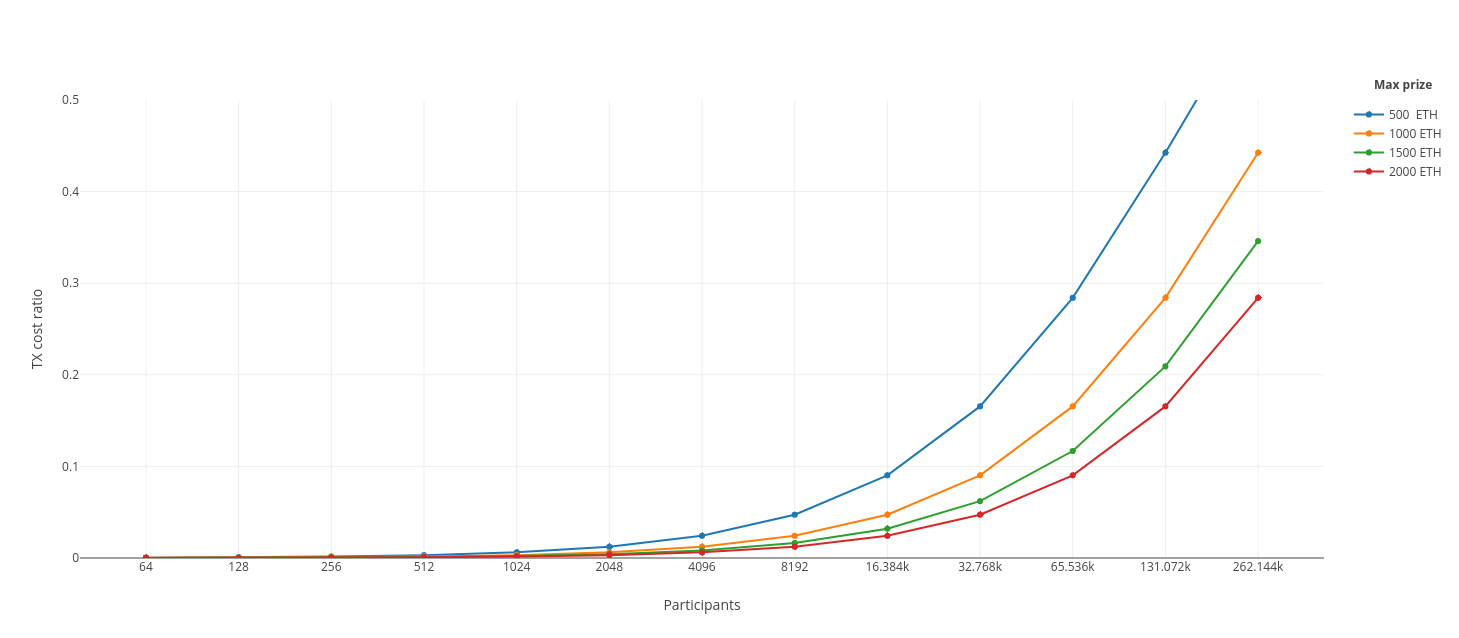
\includegraphics[width=\columnwidth]{figures/max_participants_cost_ratio.png}
  \caption{Cost ratio as a function of participants and max prize.}
  \label{fig:cost-ratio-chart}
\end{figure}

\begin{figure}[htbp]
  \centering
  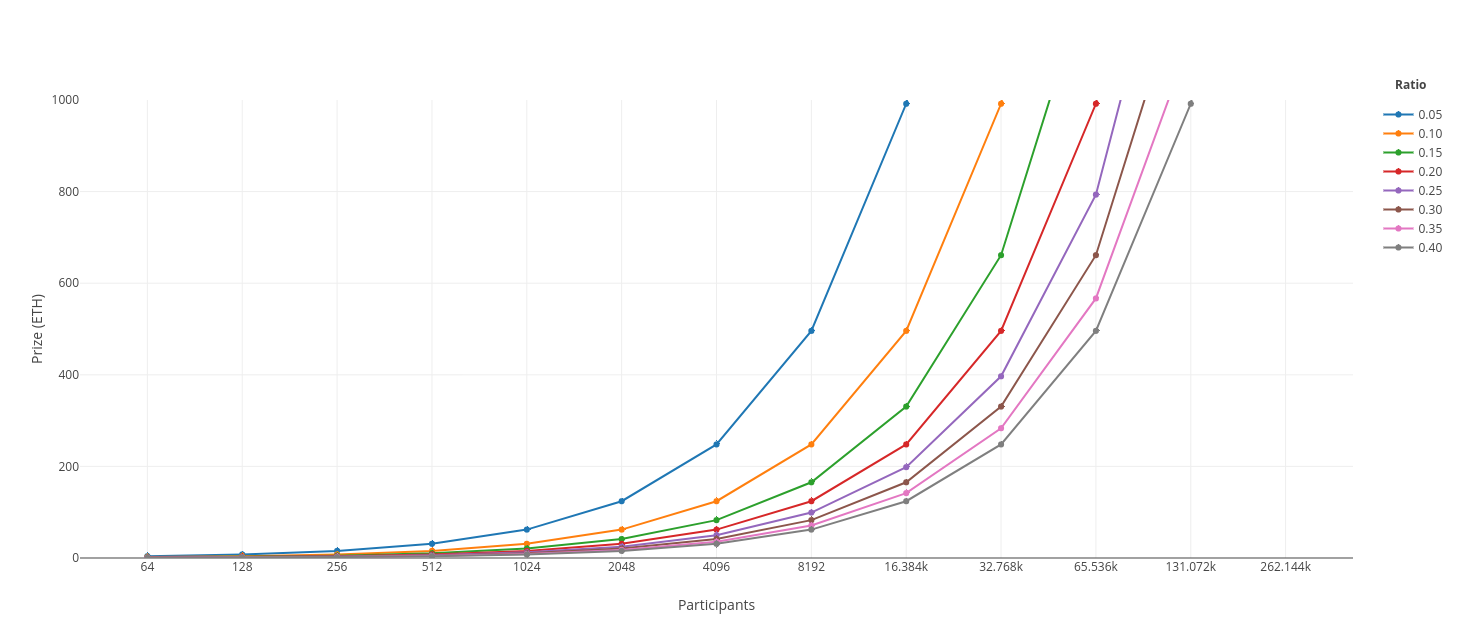
\includegraphics[width=\columnwidth]{figures/max_participants_prize.png}
  \caption{Prize as a function of participants and cost ratio.}
  \label{fig:prize-chart}
\end{figure}

\begin{figure}[htbp]
  \centering
  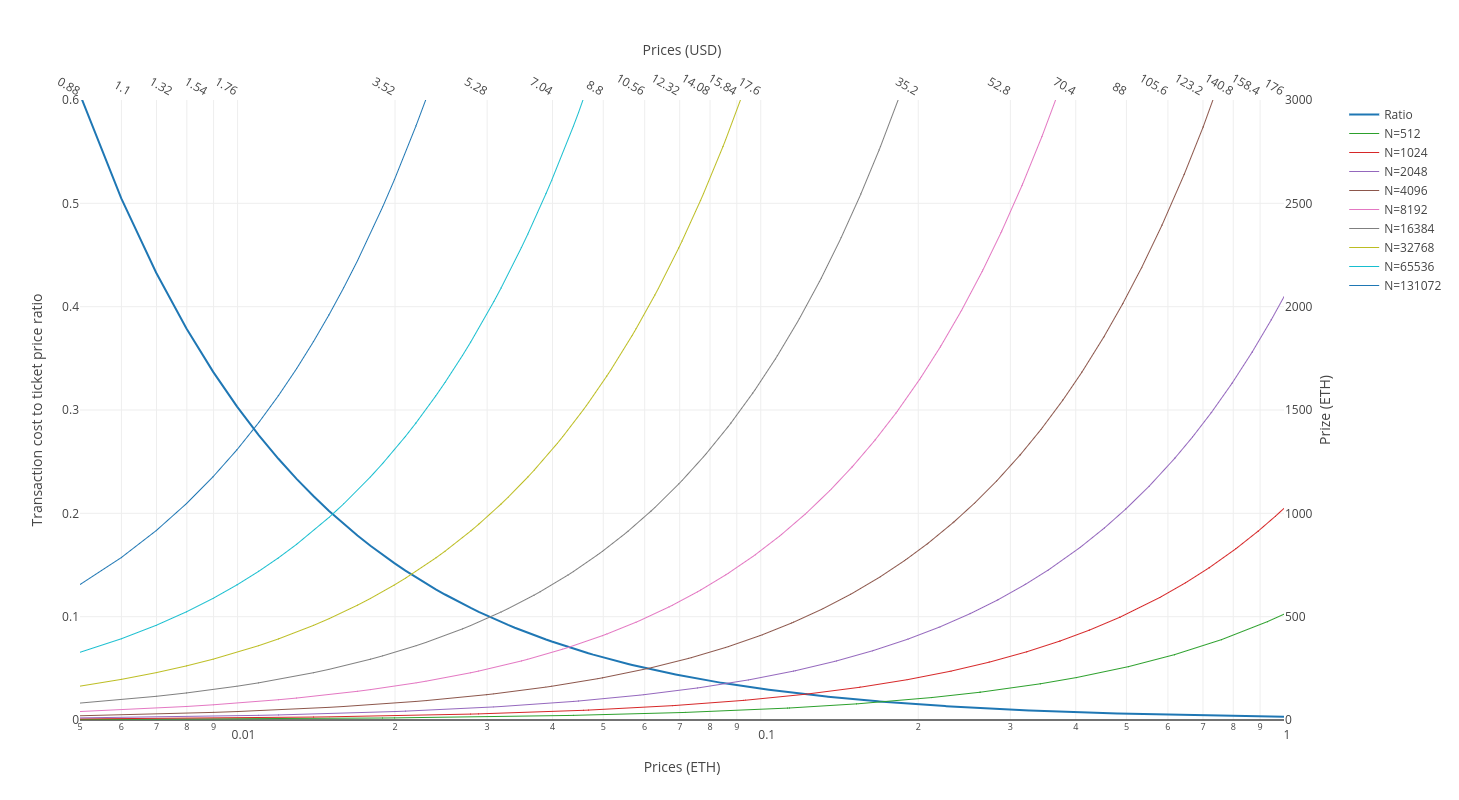
\includegraphics[width=\columnwidth]{figures/ticket_prices.png}
  \caption{Cost ratio and prize as a function of participants and ticket price.}
  \label{fig:price-chart}
\end{figure}

\section{Analysis}
\label{sec:analysis}

\subsection{Consequences of interactivity}

Based on the implementation choices of the lottery and the above results and discussion, it is possible to get an insight into important properties and trade-offs of the lottery. The lottery is interactive in that participants have to make several transactions in order to complete it successfully. The interactivity is a trade-off made in this design, as opposed to that of \cite{andrychowicz_secure_2014,bentov_how_2014}, where fewer transactions are necessary, but an upfront deposit is needed from all participants. We found that in our design, this has consequences for the scalability for several reasons. One is that the amount of transactions needed to play the lottery will be so high that it will start to congest the entire Ethereum network. Another reason is that the transaction costs put a lower bound on the minimum viable ticket price. As we operate with a maximum lottery prize for security reasons, this means that lotteries with higher ticket prices will have less capacity for participants.

What is gained by the interactivity of the scheme is that the lottery will complete as long as just one player follows the rules. Deposits are not needed as it seems a player has nothing to gain by not following the rules. A collusion of participants will not be able to predict the outcome of the randomness other than the outcome of the matches between players in the collusion. Due to secrets being committed to and not revealed until both players of a match have finalized their commitments, a collusion will not have any advantage over a single honest player.

We found that it is the cost of setting up the lottery by deploying contracts that is the most significant transaction cost. Since this cost directly influences the minimum viable ticket price, reducing the transaction cost of setting up the lottery would make the lottery capable of having more participants. It is likely that reducing the transaction cost can be done by using different design patterns in the smart contracts. Simply optimizing the length of the variables will also save some transaction costs. The current implementation only uses \texttt{uint256} types for numbers, but most of the numbers will never be so big that they need 256 bits to represent them.

The number of transactions needed to play the lottery has consequences both for the scalability of the lottery and the total transaction cost. This number can be reduced by playing the digital coin tosses \emph{off-chain}. Off-chain means that some part of a protocol is handled between the players over another communication channel than directly on the blockchain. Consider the digital coin toss after the commitments are made. As the outcome at that point is determined if both players reveal their secrets, it's not actually necessary to do that on the blockchain. The players could simply reveal their secrets to each other in private, and then one player would not have to make an actual transaction, as the losing party would not gain anything but still pay a transaction fee. If only the winner makes a reveal transaction, they will win regardless of what the loser does. Doing this requires no change in the smart contracts from what they are in the current implementation. 

It is possible that this idea of negotiating the matches off chain could be taken even further by using hierarchical deterministic secrets (HDS) \cite{wuille_bitcoin_2012}. The idea is that participants make a single commitment to a public key at the beginning of the tournament. In each match of level $i$, players derive a private key of index $i$ from the committed public key. This private key will serve as the secret in a normal digital coin toss protocol. The way HDS work is that a parent asymmetric key pair $(SK_p, PK_p)$ can generate deterministic key child key pairs with specific indices. By knowing just the public parent key, one can generate child public keys $\{PK_0, ..., PK_i\}$, and by knowing the private parent key, one can generate child private keys $\{SK_0, ..., SK_i\}$ which correspond to public keys with the same index. This means that a single public key can serve as a series of commitments by using its child public keys. The secrets will be verifiable as it is possible to verify that a private key corresponds to a public key if one knows both. Using this idea, a lottery could be negotiated off-chain once all players have made their commitments. Since it must be necessary to enforce the rules in case participants do not engage in the off-chain negotiation, all the contracts in the tournament would still have to exist, but would not necessarily be used. If commitments are made during the purchasing phase, the spike in transaction demand when playing the first matches could be drastically be reduced, hence increasing the scalability of the lottery.

\subsection{Tournament without a full binary tree}

The design of the lottery uses a tournament that is required to be a full binary tree and to be set up before players join. This limits the amounts of players in the lottery to those that is a power of two. While this limitation might make the lottery impractical, it makes it easier to reason about its properties in theory. If one were to allow for more flexible amounts of participants by allowing a non-full binary tree in the tournament, one would have to make sure that players would still have the same probability of winning. For instance, if one handles a tournament with $2^L+1$ players by having one player in a separate subtree, that player would advance to the final match without playing a single match before that. Should that player then be eligible for a smaller prize, or pay a higher ticket price?

Another possible solution is to have some matches consisting of three players instead of just two. Unfortunately, due to the time limits, this can give an advantage to two players in the same match colluding. In a match with three players, each player would ideally have a $\frac{1}{3}$ probability of winning, so that in a match with two colluding players, they would have a $\frac{2}{3}$ probability of winning. But if the secret of the non-colluding party Alice is revealed first, the colluding parties Colin and Lucy have three options. (i) Only Colin reveals, (ii) only Lucy reveals, and (iii) both reveal. Assuming each player who reveal has an equal probability of winning and that their secrets are uniformly random, the first two options each have a $\frac{1}{2}$ probability of either Colin or Lucy winning, while in the third options there's a $\frac{2}{3}$ chance of either winning. The slim probability that Alice wins in all the three options is just $\frac{1}{2 \cdot 2 \cdot 3}=\frac{1}{12}$, making the either Carol or Lucy win in 11 of 12 cases.

It is possible that there is a design in which a tournament with any amount of participants can be played fairly, but it would involve some considerable design changes from our lottery that is beyond the scope of this thesis.

\subsection{Mitigating a censorship attack}
\todo{It might be too hard to do something about this, actually.}

A possible vulnerability in censorship of transactions was discovered. Even though the risk of a censorship attack is unknown, if we assume the possibility of a miner or collusion of miners with a majority hashing power, it would at some size of the lottery prize be in their economic interest to launch such an attack. A censorship attack is possible because of the time limits of matches, because a player unable to make transactions will lose. The time limits are however necessary to prevent a single participant halting the entire process. 

A possible way of mitigating a censorship attack is to annul the result of the tournament if the winner won a certain fraction of their matches by forfeiture. This could possibly do some collateral damage in that an honest winner could risk being suspected of cheating. It could also make the off-chain negotiation mentioned earlier in this section impractical. 

\chapter{Discussion}
\label{chap:discussion}

% The results you have collected and the process you when through to develop the project have been presented earlier. This Chapter is used to talk about your interpretations of results or the process. It might be a discussion of the language you used. A tool that you started to use but then stopped using for some reason. It could give insight into the evolution of your process.

\section{Programming tools}
\label{sec:tools}

We were generally able to use existing tools to our advantage for development and simulation. Truffle was used to compile and manage smart contracts. We used Truffle's testing environment and smart contract abstraction to successfully run unit tests and simulations on our code. Ganache is a program that starts an Ethereum RPC server and blockchain on your local computer. This allows one to quickly deploy contracts, make transactions, mock behaviour, and measure performance without using something out of the developer's control such as the Ethereum mainnet or even a testnet.

By limiting ourselves to using the smart contract abstraction that comes with Truffle, we were not able to overcome some shortcomings when simulating and testing. Truffle's smart contract abstraction is designed to be used in web clients of dApps that interact with the Ethereum blockchain. Since each interaction with the blockchain involves an RPC, such interactions are handled with JavaScript promises – a language feature that facilitates making asynchronous applications. For every transaction RPC that is made, Truffle will wait until it is confirmed in the blockchain before it performs the next RPC. This limits how we can use Truffle when simulating, as a simulation may involve thousands of transactions, many of which can be made in parallel. In our code, we have to wait for each transaction to be confirmed before the next one is made. As our simulations require some transactions to be made in specific order, such as making commitments before revealing secrets, we have to use promises in some cases. We could avoid this limitation by making all our transaction RPCs by using web3js directly, but that would involve a more complicated simulation program. This limited out simulations to use no more than 512 participants, as using more would take a long time. However, we don't think simulations with more participants would provide much more useful data.

Our smart contracts are highly dependent on timing conditions. The time limits are specified in fields that denominate block height. E.g. a match contract is initialized with three limits: \texttt{tCommit}, \texttt{tReveal}, and \texttt{tPlay}. These are essential for security in a real deployment, but testing and simulating with many time conditions can be hard. In our testing environment we run a local blockchain using Ganache. Due to the issue with Truffle discussed above, we have to enablea feature called \emph{auto mining} with Ganache, so that a new block is generated with each transaction. This is not how the blockchain would behave in a live situation, so instead of altering our smart contract code to fit into our testing environment, we chose to not use time limits in the contracts when testing and simulating. We could configure a much more complicated testing environment where we can control which transactions are mined which which block heights etc., but chose to not spend time doing it as we were nonetheless able to run useful simulations and tests. 

\section{Blockchain security}
\label{sec:discussion-security}

The common security assumptions, attack vectors, and threat models of the underlying blockchain can be essential to understand and consider when deploying applications on top of the blockchain. Blockchain security, however, is a complex and not well understood topic. Researchers and practitioners in the space have identified various attack scenarios and concerns related to the security of a blockchain. We have discussed some of these, such as selfish mining, censorship, and block reorganization. We consider these issues important to discuss when developing an application on top of a blockchain, but since we lack real data on what happens during such an attack, as it has not happened on a major blockchain, discussing it is somewhat speculative.

Our analysis on the security of our implementation is based on uncertain assumptions and speculative attack scenarios. While something like censorship of transactions by miners certainly is possible, there is no research indicating that it is common or even in miners' interest to do so. On the other hand, blockchain platforms for smart contracts is a relatively new phenomenon, so it may well be a latent threat that will be a concern in the future. While we think that discussion on theoretical attacks is useful, we admit that the results from such discussion cannot give a concrete results that are applicable in all cases. However, when designing protocols that handle large amounts of money, a prudent approach should be taken as it's better to fail on the side of being too cautious rather than too reckless. With that in mind, our analysis on potential attacks is indeed useful. 

\section{Experimentation}
\label{sec:experimentation}

Experimentation within a real setting is something we were not able to do in this thesis. The plan was to only make a proof-of-concept implementation, but the lack of experience from a real deployment makes it difficult to answer whether Ethereum is a good platform for a distributed lottery. While some properties of the blockchain and applications built on top of it can be analyzed by merely using theory and assumptions, the live version of a blockchain like Ethereum is a complex system with many stakeholders and participants, many of whom are opportunistic or right out adversarial. One infamous example of something unexpected going wrong is the DAO and reentrancy bug exploit which resulted in a hardfork of Ethereum \cite{dhillon_dao_2017}. 

Not only is a dApp likely to face unexpected issues when deployed on a live network, but users of the dApp might have various expectations and mental models that can make a theoretically sound app not usable by its intended users. There are to date few actively used dApps on any smart contract platform, and this might be because of a failure to communicate the platform's advantages to the broader audience. Our lottery scheme is an interactive one where users are required to be online and send transactions over a period of time, and possibly enact countermeasures to attacks by adversaries. This is much more complicated than traditional online gambling sites where one typically performs one transaction and is then automatically able to withdraw the potential earnings. 

\chapter{Conclusion}
\label{chap:conclusion}

% This is where you provide an overview of the thesis now that it is finished. What are the critical things that can be learnt from the thesis for the reader.

The work of this thesis has been to implement a distributed lottery in Ethereum and analyze its properties and viability by gathering data through simulations and discussing adversarial threats. We found that the lottery specified in \cite{miller_zero-collateral_2017} can easily be implemented in smart contracts on Ethereum. We found that transaction costs can be reduced by 36\% by splitting code into two separate match contracts, and that additional savings can probably be made by deduplicating code. Our implementation is possible to deploy on the Ethereum platform by using scripts and the Truffle framework.

Simulations of setting up and playing the lottery were executed on a local Ethereum blockchain to get insight into gas usage and whether our proof-of-concept implementation worked as expected. We found that the implementation does work as expected on a local blockchain, but attempts to deploy it on a global blockchain were not made. Gas usage was dominated by the smart contract deployment transactions needed to set up the lottery, which is all paid for by the lottery organizer. From this fact we assume that the lottery is viable only if the lottery organizer can take a fee of the total price which at least covers the expense from setting it up. Based on the transaction costs, we found a way to estimate a minimum ticket price for as a function of gas price and organizer fee.

Taking the current transaction throughput of the Ethereum blockchain into account, we found a limit to how many participants a lottery of this type is able to handle if it is to finish within a reasonable time period. This limit can be expressed as a linear function of the duration of the lottery, the number of transactions in each block, and the ratio of total transactions on Ethereum are addressed to the lottery. By setting the time limit to a couple of days and assuming that 10\% of all transactions are related to the lottery, we found the limit to be in the order or 100000s of participants or $2^{17}$.

The security of the lottery was discussed in the context of several known attack vectors for blockchain applications and web applications. We found that censorship of transactions from a powerful collusion of miners is likely to be the most concerning. Due to the interactivity and time limits of the lottery protocol, we found that if miners successfully block transactions from one account for each level of the tournament, they have the power to select an arbitrary participant to win the entire lottery.
We discussed mitigating this issue, but were unable to find a satisfactory solution other than not playing the lottery with high stakes if there is a powerful miner collusion. 

A truncated version of this work was submitted to the \textbf{2nd international workshop on future perspective of decentralized applications 2019} and is at the time of submitting this thesis awaiting review.

\section{Future work}
\label{sec:future-work}

We have identified several directions for further research on implementing lotteries on smart contact platforms.

\subsection{Minimizing transaction costs}

We were able to reduce gas usage by 36\% by splitting up the match contract to two separate contracts. As we mentioned earlier, it should be possible to reduce gas usage even further by deduplicating code by using patterns such as library contracts and proxy contracts. As of our implementation, the organizer has to take a risk when setting up the lottery, as there is a chance the lottery will fail to start by not enough participants joining. By reducing transaction costs, the potential losses from this risk will be lower.

\subsection{Minimizing interactivity}

The lottery implemented in this thesis requires participants to interact by sending transactions several times. Other blockchain lottery schemes such those described in \cite{andrychowicz_secure_2014} and \cite{bentov_how_2014} require less interaction, but do need a high deposit from all players. In our discussion on security we identified a vulnerability in attacks from miners censoring transactions. We also found that with the current transaction throughput in Ethereum, our lottery will need a very long time to finish if it scales to hundred of thousands of participants. 

It might be possible to come up with a design that both require few interactions and does not need high deposits from participants to avoid halting. Since security is a high priority requirement when handling large amounts of money, such a design would be a welcome contribution.

\subsection{Off-chain negotiation}

Even though the smart contracts in our lottery must have the capability of enforcing the protocol, they don't necessarily need to process all the transactions as we laid out. In order to reduce gas usage and number of interactions, matches can be negotiated between opponents off-chain. E.g. when both players have made their commitments, they can reveal their secrets over another communication channel. By seeing one's opponent's secret, one knows what the outcome of the match will be if both players were to reveal the secret on the blockchain. Instead, only the winner can reveal their secret while the loser forfeits by not making the reveal transaction.

Even though gas usage from interacting with the match contracts isn't that high, reducing it would nonetheless reduce overall transaction costs and make the lottery more viable. It would also be interesting to explore if hierarchical deterministic secrets could be used to avoid making a commitments for each match. HDS is a scheme where a private key can generate child private keys and a corresponding public key can generate child public keys. Since the algorithm used is deterministic, the generated secrets can possibly be verified at a later stage. While the original HDS scheme proposed in \cite{wuille_bitcoin_2012} might be unfit for the purpose, as leaked child keys can make it possible to derive the parent private key, the scheme proposed in \cite{gutoski_hierarchical_2015} does not have this vulnerability and might be better suited.

\subsection{Formal analysis of security}

While we have discussed security issues in this thesis, we believe an even more rigorous analysis is possible. As the blockchain space matures, more research and experience is likely to appear in the coming years. This can be used to arrive at better estimates on what assumptions and conditions that are needed to make our lottery secure. Perhaps most important is more knowledge on the topic of censorship of transactions. Both models that allow us to find under what conditions censorship is likely, as well as tactics to avoid censorship would be interesting.




\ifthenelse{\boolean{HarvardCitations}}{%
	\bibliographystyle{agsm} % used for Harvard style references. Names - Humanities & Interaction Design
}{%
	\bibliographystyle{ntnuthesis/ntnuthesis} %used for Vancouver style references. Numbers - Computer Science & Physics
}

\bibliography{bibliography}

\appendix
\chapter{Listings}
\label{appendix:listings}

\section{Solidity contracts}

\subsection{Abstract match contract}
\lstinputlisting[language={Solidity}, caption={Full Solidity contract for AbstractLotteryMatch.}, label={lst:FullAbstractLotteryMatch.sol}]{listings/FullAbstractLotteryMatch.sol}

\subsection{First level match contract}
\lstinputlisting[language={Solidity}, caption={Full Solidity contract for FirstLevelMatch.}, label={lst:FullFirstLevelMatch.sol}]{listings/FullFirstLevelMatch.sol}

\subsection{Internal match contract}
\lstinputlisting[language={Solidity}, caption={Full Solidity contract for InternalMatch.}, label={lst:FullInternalMatch.sol}]{listings/FullInternalMatch.sol}

\subsection{Master contract}
\lstinputlisting[language={Solidity}, caption={Full Solidity contract for LotteryMaster.}, label={lst:FullLotteryMaster.sol}]{listings/FullLotteryMaster.sol}

\section{Javascript}

\subsection{Simulate lottery setup}
\lstinputlisting[language={ES6}, caption={Truffle test suite for simulating lottery setup.}, label={lst:SimulateLotterySetup.js}]{listings/SimulateLotterySetup.js}

\subsection{Simulate lottery play}
\lstinputlisting[language={ES6}, caption={Truffle test suite for simulating lottery play.}, label={lst:SimulateLotteryPlay.js}]{listings/SimulateLotteryPlay.js}

\chapter{Simulation data}
\label{appendix:simulation-data}

\section{Gas usage}
\label{sec:simulation-results}

\subsection*{Steps to replicate}
Using Git repository located at~\url{https://github.com/viktorfa/lottery-truffle.git}. Dual match simulations from Git commit \texttt{36ee7818}. Single match simulations from Git commit \texttt{63747577}. Variable \texttt{L} in \texttt{tests/Lottery.simulate.js} set to {8} for both simulation suites. Simulations run with command \texttt{truffle test ./test/Lottery.simulate.js} with a Ganache Ethereum RPC client running.

\subsection*{Results}

\begin{table}[h]
\centering
\caption{Statistics from dual match simulation with 256 participants.}
\begin{tabular}{|l|l|l|l|l|l|}
\hline

Stats n=5 &  &  &  &  &  \\ \hline
Contract & Method & Mean & Stdev & Range & Stdev/Mean \\ \hline
FirstLevelMatch & commit & 76611 & 0 & 0 & 0 \\ \hline
FirstLevelMatch & reveal & 42883 & 0.8367 & 1.25 & 0.00001951 \\ \hline
InternalMatch & commit & 88672 & 2.51 & 7 & 0.00002831 \\ \hline
InternalMatch & reveal & 42883 & 1.673 & 4 & 0.00003902 \\ \hline
LotteryMaster & deposit & 73925 & 0 & 0 & 0 \\ \hline
LotteryMaster & setFinalMatch & 49282 & 0 & 0 & 0 \\ \hline
LotteryMaster & withdraw & 39171 & 5.477 & 10 & 0.0001398 \\ \hline
Deployments &  &  &  &  &  \\ \hline
FirstLevelMatch &  & 1693715 & 28.62 & 64 & 0.0000169 \\ \hline
InternalMatch &  & 1697002 & 1830 & 1026 & 0.0010785 \\ \hline
LotteryMaster &  & 1693664 & 0 & 0 & 0 \\ \hline
Total set up &  & 433555262 & 3534 & 2288 & 0.00000815 \\ \hline
Total set up and play &  & 516524423 & 3428 & 2917 & 0.00000664 \\ \hline

\end{tabular}
\end{table}


\end{document}
